%%%%%%%%%%%%%%%%%%%%%%%%%%%%%%%%%%%%%%%%%%%%%%%%%%%%%%%%%%%%%%%%%%%%%%%
% Latex file abstraction to skripsi class
%%%%%%%%%%%%%%%%%%%%%%%%%%%%%%%%%%%%%%%%%%%%%%%%%%%%%%%%%%%%%%%%%%%%%%%
\documentclass{skripsi}

% ------------------------------------------------------------
% Add your own needed package here
% ------------------------------------------------------------
% Needed to add prefix for images and tables
\usepackage[titles]{tocloft}
\renewcommand\cftfigpresnum{Gambar\  }
\renewcommand\cfttabpresnum{Tabel\   }

% Needed to add hyperlink to the document
\usepackage{hyperref}
\newlength{\mylenf}
\settowidth{\mylenf}{\cftfigpresnum}
\setlength{\cftfignumwidth}{\dimexpr\mylenf+2em}
\setlength{\cfttabnumwidth}{\dimexpr\mylenf+2em}

% Needed to add caption
% - labelfont: caption label
% - font: caption content
% - labelsep: caption separator
\usepackage[center,labelfont=bf,font=bf,labelsep=space]{caption}
% Needed to add ability to customize subcaption
\usepackage{subcaption}

% Needed to force placing figure here
\usepackage{float}
\usepackage{csquotes}
% Needed to put paragraph inside itemize
\usepackage{enumitem}
% Needed to add ability for sub-sub-subsection
\usepackage{titlesec}

% Needed to make `\paragraph' behave like `\subsubsubsection'
\titleformat{\paragraph}
{\normalfont\normalsize\bfseries}{\theparagraph}{1em}{}
\titlespacing*{\paragraph}
{0pt}{3.25ex plus 1ex minus .2ex}{1.5ex plus .2ex}

% Needed to remove orphan and widowG
% FIXME didn't work
\usepackage[all]{nowidow}

% Needed to avoid overfull in table
\usepackage{ragged2e}
\usepackage{longtable, makecell}
\newcolumntype{L}[1]{>{\RaggedRight}p{#1}}
\renewcommand\theadfont{\small\bfseries}
\setcellgapes{3pt}

% Needed to use <x>cm in table size
\usepackage{array}
\newcolumntype{P}[1]{>{\raggedright\let\newline\\\arraybackslash\hspace{0pt}}p{#1}}

% -----------------------------------------------------------------
% Custom source code style
% -----------------------------------------------------------------
\usepackage{listings}
\usepackage[newfloat,chapter]{minted}

% allow caption and label in minted
% https://tex.stackexchange.com/questions/254044/caption-and-label-on-minted-code
\newenvironment{code}{\captionsetup{type=listing}}{}
\SetupFloatingEnvironment{listing}{name=Tabel Kode}

\usepackage{tcolorbox}
\tcbuselibrary{listings,minted,skins,breakable}
\usetikzlibrary{decorations.pathmorphing}
\usetikzlibrary{decorations.pathreplacing}
\newtcblisting{ignasicblock}[1][]{%
  breakable,
  colback=white,
  colframe=black,
  colbacktitle=white,
  sharp corners,
  enhanced,
  listing engine=minted,
  listing only,
  left=10mm,
  title=Source Code,
  halign title=center,
  overlay={\draw[line width=.5mm] ([xshift=8mm]frame.south west)
    -- ([xshift=8mm]frame.north west);
    \node[right] at (title.west) {No};},
  minted style=colorful,
  minted language=Python,
  minted options={%
    linenos=true,
    fontsize=\footnotesize,
    numbersep=6mm,
    texcl=true,
    breaklines=true,
    autogobble=true},
  coltitle=black,
  #1
}

% Ability to draw overlay braces on tcolorbox
% Big thanks for Thomas F. Sturm
\newcommand{\drawbrace}[5][]{%
  \draw [decorate,decoration={brace,amplitude=5pt},blue!75!black,line width=1pt]
    ([xshift=#2,yshift=-3.3mm-#3*12pt]interior.north west)
    -- ([xshift=#2,yshift=-2.7mm-#4*12pt]interior.north west)
    node [align=center,right=10pt,midway,circle,draw=blue!50,fill=blue!5,text=black,
      font=\sffamily\small,#1] {#5};
}

% Ability to draw overlay line on tcolorbox
\newcommand{\drawline}[5][]{%
  \draw [blue!75!black,line width=1pt]
    ([xshift=#2,yshift=-3mm+6pt-#4*12pt]interior.north west)
    -- ([xshift=#3,yshift=-3mm+6pt-#4*12pt]interior.north west)
    node [align=center,right=5pt,circle,draw=blue!50,fill=blue!5,text=black,
      font=\sffamily\small,#1] {#5};
}

\definecolor{codebg}{rgb}{0.95,0.95,0.95}
\renewcommand\theFancyVerbLine{\footnotesize\arabic{FancyVerbLine}}

% -----------------------------------------------------------------
% Font style
% -----------------------------------------------------------------
\usepackage{fontspec} % use custom font

\setmainfont[Path=/path/to/your/calibri/font/,
    BoldItalicFont=calibriz.ttf,
    BoldFont      =calibrib.ttf,
    ItalicFont    =calibrii.ttf]{calibri.ttf} % use original calibri font

\setmonofont[Path=/path/to/your/courier/font/,
    BoldItalicFont=courbi.ttf,
    BoldFont      =courbd.ttf,
    ItalicFont    =couri.ttf]{cour.ttf} % use original courir new font

% -----------------------------------------------------------------
% Debungging configuration
% -----------------------------------------------------------------
%\overfullrule=2cm % show overfull
%\usepackage{showframe} % show frame margin
%\renewcommand\ShowFrameLinethickness{0.25pt}
%\renewcommand*\ShowFrameColor{\color{red}}


% -----------------------------------------------------------------
% Bibliography style
% -----------------------------------------------------------------
%%%%%%%%%%%%%%%%%%%%%%%%%%%%%%%%%%%%%%%%%%%%%%%%%%%%%%%%%%%%%%%%%%%%%%%
% This file redefine reference list to match Harvard-Angila flavor
% Great thanks for Moritz (moewe) Wemheuer
%%%%%%%%%%%%%%%%%%%%%%%%%%%%%%%%%%%%%%%%%%%%%%%%%%%%%%%%%%%%%%%%%%%%%%%

\usepackage[
  backend=biber,
  style=ext-authoryear-comp, giveninits, uniquename=init, maxbibnames=999,
  urldate=long,
  innamebeforetitle, articlein=false,
]{biblatex}

% 1.2
\DeclareDelimFormat*{nameyeardelim}{\addcomma\space}
\DeclareDelimFormat[textcite]{nameyeardelim}{\addspace}

% 2.5
\DeclareDelimFormat{andothersdelim}{\addcomma\space}

% 2.7
\renewcommand*{\compcitedelim}{\multicitedelim}

% 2.8
\makeatletter
\AtEveryCitekey{\global\undef\cbx@lastyear}
\makeatother

% ignore 2.10 for the time being

% 4.1
\DeclareNameAlias{sortname}{family-given}
\DeclareFieldFormat{biblabeldate}{#1}
\DeclareFieldAlias{biblistlabeldate}{biblabeldate}

% 4.3
\DeclareDelimFormat{editortypedelim}{\addspace}
\DeclareDelimFormat{translatortypedelim}{\addspace}

% 4.4
\DeclareFieldFormat
  [article,inbook,incollection,inproceedings,patent,thesis,unpublished]
  {title}{#1\isdot}

% as for the year of the chapterv vs year of the book in 4.4
% I have never seen such a distinction and in general I imagine
% it would be quite hard to find out the year of a chapter
% in a collection work since only the year of the collection is given
% I imagine that in practice you would almost always end up douplicating
% the year.

% 4.8 & 5.11
\DefineBibliographyStrings{english}{
  urlfrom   = {available at},
  urlseen   = {accessed},
  bathesis  = {BA},
  mathesis  = {MA},
  phdthesis = {PhD},
}
\newcommand*{\mkbiburlangle}[1]{<#1>}
% or {<#1>}
% or {\ensuremath{\langle}#1\ensuremath{\rangle}}
% or {guilsinglleft#1\guilsingleright}
\DeclareFieldFormat{url}{\bibstring{urlfrom}\addcolon\space \mkbiburlangle{\url{#1}}}
\DeclareFieldFormat{urldate}{\mkbibbrackets{\bibcpstring{urlseen}\space#1}}

% 4.9
\renewcommand*{\jourvoldelim}{\addcomma\space}
\renewcommand*{\volnumdelim}{}
\DeclareFieldFormat[article,periodical]{number}{\mkbibparens{#1}}

\renewcommand*{\volnumdatedelim}{\addcomma\space}
\DeclareFieldFormat{issuedate}{#1}

% 4.12 :-(
% note that I used the new preferred resolver https://doi.org/
% instead of http://dx.doi.org/
\DeclareFieldFormat{doi}{\url{https://doi.org/#1}}

\addbibresource{daftar-pustaka.bib}

% Needed t % change `and' to `&'&
\renewcommand*{\finalnamedelim}{%
  \ifnumgreater{\value{liststop}}{2}{\finalandcomma}{}%
  \addspace\&\space}

% Needed to remove space in generated documents if we put comments in
% source
\newcommand{\cmmnt}[1]{\ignorespaces}

% -----------------------------------------------------------------
% Fill your data here
% -----------------------------------------------------------------
% title
\titleskripsi{The Compendious Book on Calculation by Completion and Balancing}
% personal data
\fullname{M. Ibn Musa al-Khwarizmi}
\idnum{112233445566}
\approvaldate{N/A}
\degree{N/A}
\yearsubmit{2019}
\dept{TEKNIK INFORMATIKA}
\faculty{FAKULTAS ILMU KOMPUTER}
\university{universitas brawijaya}
\city{malang}
% supervisor data
\firstsupervisor{Nama Dosen Pembimbing I, S.T., M.T., Ph.D}
\firstsupervisornip{NIP: 1234 45679}
\secondsupervisor{Nama Dosen Pembimbing II, S.T., M.T., Ph.D}
\secondsupervisornip{NIP: 5555 7777}

% -----------------------------------------------------------------
% And so it begins
% -----------------------------------------------------------------
\begin{document}

% -----------------------------------------------------------------
% Cover
% -----------------------------------------------------------------
\cover

% -----------------------------------------------------------------
% Approval Page
% -----------------------------------------------------------------
%\preapprovalpage
\approvalpage

%-----------------------------------------------------------------
% PERNYATAAN ORISINALITAS
%-----------------------------------------------------------------
{\orisinalitas

  Saya menyatakan dengan sebenar-benarnya bahwa sepanjang pengetahuan
  saya, di dalam naskah skripsi ini tidak terdapat karya ilmiah yang
  pernah diajukan oleh orang lain untuk memperoleh gelar akademik di
  suatu perguruan tinggi, dan tidak terdapat karya atau pendapat yang
  pernah ditulis atau diterbitkan oleh orang lain, kecuali yang secara
  tertulis disitasi dalam naskah ini dan disebutkan dalam daftar
  referensi.

  Apabila ternyata didalam naskah skripsi ini dapat dibuktikan
  terdapat unsur-unsur plagiasi, saya bersedia skripsi ini digugurkan
  dan gelar akademik yang telah saya peroleh (sarjana) dibatalkan,
  serta diproses sesuai dengan peraturan perundang-undangan yang
  berlaku (UU No. 20 Tahun 2003, Pasal 25 ayat 2 dan Pasal 70).
  \vspace{1.5cm}

  \noindent
  \hspace*{8cm}Malang, 2 Juli 2019   \vspace{2.5cm}   \\

  \hspace*{7cm}\underline{M. Ibn Musa al-Khwarizmi} \\
  \hspace*{8cm}NIM : 112233445566
}

%-----------------------------------------------------------------
% Disini awal masukan untuk Prakata
%-----------------------------------------------------------------
{\preface

  Puji syukur kehadirat Allah SWT yang telah melimpahkan rahmat,
  taufik dan hidayah-Nya sehingga skirpsi yang berjudul ``The Compendious Book
  on Calculation by Completion and Balancing'' ini dapat terselesaikan. Dengan
  selesainya penulisan skirpsi ini, penulis ingin menyampaikan terima kasih
  kepada:

  \begin{singlespace}
    \begin{enumerate}
  \item{Allah SWT yang telah memberikan nikmat kesehatan, kekuatan dan
      kemudahan sehingga penulis dapat menyelesaikan skripsi ini.}
  \item{Ustaz, orang tua dan seluruh keluarga besar penulis yang
      senantiasa mendoakan dan mendukung demi terselesaikannya skripsi
      ini.}
  \item{Bapak Nama Dosen Pembimbing, S.T., M.T., Ph.D, selaku Dosen Pembimbing I
      yang telah meluangkan waktu untuk membimbing dengan semangat dan
      sabar sehingga penulis dapat menyelesaikan skripsi ini.}
  \item{Bapak Nama Dosen Pembimbing, S.T., M.T., Ph.D, selaku
      Dosen Pembimbing II yang telah mengarahkan dan membimbing
      penulis dengan dengan semangat dan sabar sehingga penulis dapat
      menyelesaikan skripsi ini.}
  \item {Bapak Tri Astoto Kurniawan, S.T, M.T, Ph.D dan Bapak Agus
      Wahyu Widodo, S.T, M.Cs selaku Ketua Jurusan Teknik Informatika
      dan Kepala Program Studi Teknik Informatika Fakultas Ilmu
      Komputer, Universitas Brawijaya.}
  \item{Seluruh pengembang kakas bantu perangkat lunak bebas yang
      digunakan dalam skripsi ini.}
  \item{Seluruh civitas akademika Teknik Informatika Universitas
      Brawijaya yang telah banyak memberi bantuan dan dukungan selama
      penyelesaian skripsi ini.}
  \end{enumerate}
  \end{singlespace}

  Penulis menyadari bahwa dalam penelitian ini masih banyak
  kekurangan. Oleh karena itu, saran dan kritik yang membangun sangat
  penulis harapkan. Akhir kata penulis berharap penelitian ini dapat
  membawa manfaat bagi semua pihak yang menggunakannya.

  \vspace{0.8cm}

  \noindent
  \hspace*{8cm}Malang, 2 Juli 2019  \vspace{1.5cm} \\

  \hspace*{6.8cm}Penulis \\
  \hspace*{8cm}alKhwarizmi@student.ub.ac.id
}

% -----------------------------------------------------------------
% ABSTRAK INDONESIA
% -----------------------------------------------------------------
{\abstractind

  \noindent
  Lorem ipsum dolor sit amet, consectetur adipiscing elit. Proin quis magna nec
  eros hendrerit rhoncus. Mauris aliquam erat lobortis, bibendum libero nec,
  accumsan arcu. Cras eleifend, orci scelerisque scelerisque congue, ex nibh
  volutpat metus, ultrices feugiat dolor ipsum quis odio. Suspendisse vel elit
  non enim pulvinar vehicula eu id odio. In viverra aliquet ex, at volutpat odio
  ultricies sed. Quisque eu tempus metus. Vestibulum ante ipsum primis in
  faucibus orci luctus et ultrices posuere cubilia Curae; Nam a rutrum nunc, ut
  egestas neque. Etiam consectetur odio et mi laoreet egestas.  Interdum et
  malesuada fames ac ante ipsum primis in faucibus. Morbi pharetra tincidunt
  viverra. Aliquam sit amet ornare lorem, sed euismod felis. Praesent eget
  tellus ac nunc efficitur efficitur et at mi. Nunc ultricies maximus nibh, a
  sollicitudin tortor laoreet eu. Fusce velit ligula, lacinia ac tempor
  ultrices, lobortis vel nunc. Pellentesque lectus nisl, cursus vitae ultrices
  sit amet, bibendum sit amet magna. Pellentesque ullamcorper enim et nisl
  mollis, id ornare nibh luctus. Nunc ut sapien augue.  Fusce rutrum eros semper
  tincidunt malesuada. Sed ut velit eu elit consequat suscipit. Integer at eros
  felis. Nulla mollis mi dolor, id lacinia sem commodo ut. Vestibulum ornare ex
  sed consectetur suscipit. Sed vehicula feugiat justo, vitae faucibus
  elit. Praesent non aliquam nulla, eget posuere orci. Nullam ultrices velit eu
  lobortis rhoncus. Suspendisse imperdiet posuere magna in sagittis. Nullam eget
  luctus lectus. Vivamus condimentum quis velit cursus vulputate. Cras nec urna
  eget arcu hendrerit condimentum non at sem. In leo
  neque, ultrices accumsan blandit rutrum, convallis sit amet ante.\\

  \noindent
  \textbf{Keywords}: \emph{Lorem ipsum},
  \emph{dolor sit amet}, \emph{consectetur}

}

% -----------------------------------------------------------------
% ABSTRAK ENGLSIH
% -----------------------------------------------------------------
{\abstracteng

  \noindent
  Lorem ipsum dolor sit amet, consectetur adipiscing elit. Proin quis magna nec
  eros hendrerit rhoncus. Mauris aliquam erat lobortis, bibendum libero nec,
  accumsan arcu. Cras eleifend, orci scelerisque scelerisque congue, ex nibh
  volutpat metus, ultrices feugiat dolor ipsum quis odio. Suspendisse vel elit
  non enim pulvinar vehicula eu id odio. In viverra aliquet ex, at volutpat odio
  ultricies sed. Quisque eu tempus metus. Vestibulum ante ipsum primis in
  faucibus orci luctus et ultrices posuere cubilia Curae; Nam a rutrum nunc, ut
  egestas neque. Etiam consectetur odio et mi laoreet egestas.  Interdum et
  malesuada fames ac ante ipsum primis in faucibus. Morbi pharetra tincidunt
  viverra. Aliquam sit amet ornare lorem, sed euismod felis. Praesent eget
  tellus ac nunc efficitur efficitur et at mi. Nunc ultricies maximus nibh, a
  sollicitudin tortor laoreet eu. Fusce velit ligula, lacinia ac tempor
  ultrices, lobortis vel nunc. Pellentesque lectus nisl, cursus vitae ultrices
  sit amet, bibendum sit amet magna. Pellentesque ullamcorper enim et nisl
  mollis, id ornare nibh luctus. Nunc ut sapien augue.  Fusce rutrum eros semper
  tincidunt malesuada. Sed ut velit eu elit consequat suscipit. Integer at eros
  felis. Nulla mollis mi dolor, id lacinia sem commodo ut. Vestibulum ornare ex
  sed consectetur suscipit. Sed vehicula feugiat justo, vitae faucibus
  elit. Praesent non aliquam nulla, eget posuere orci. Nullam ultrices velit eu
  lobortis rhoncus. Suspendisse imperdiet posuere magna in sagittis. Nullam eget
  luctus lectus. Vivamus condimentum quis velit cursus vulputate. Cras nec urna
  eget arcu hendrerit condimentum non at sem. In leo
  neque, ultrices accumsan blandit rutrum, convallis sit amet ante.\\

  \noindent
  \textbf{Keywords}: \emph{Lorem ipsum},
  \emph{dolor sit amet}, \emph{consectetur}

}

% -----------------------------------------------------------------
% TOCS
% -----------------------------------------------------------------
\tableofcontents
\addcontentsline{toc}{chapter}{DAFTAR ISI}
\listoftables
\addcontentsline{toc}{chapter}{DAFTAR TABEL}
\listoffigures
\addcontentsline{toc}{chapter}{DAFTAR GAMBAR}
% FIXME \listofappendices
\addcontentsline{toc}{chapter}{DAFTAR LAMPIRAN}

% -----------------------------------------------------------------
% Chapter
% -----------------------------------------------------------------
% change numbering to arabic from bab1
\selectlanguage{bahasa}\clearpage\pagenumbering{arabic}\setcounter{page}{1}

%%%%%%%%%%%%%%%%%%%%%%%%%%%%%%%%%%%%%%%%%%%%%%%%%%%%%%%%%%%%%%%%%%%%%%%
% BAB 1
%%%%%%%%%%%%%%%%%%%%%%%%%%%%%%%%%%%%%%%%%%%%%%%%%%%%%%%%%%%%%%%%%%%%%%%
\mychapter{1}{BAB 1 PENDAHULUAN}

\section{Latar Belakang Masalah}

\emph{Cardiovaskular disease} (CVD) atau penyakit kardiovaskular merupakan penyebab utama kematian di dunia.
Pada tahun 2019, diperkirakan terdapat 17,9 juta kematian akibat CVD \parencite{worldhealthorganizationCardiovascularDiseasesCVDs2021}.
Angka kematian tersebut mencakup sekitar 32\% dari total kematian di dunia. 
Dengan angka kematian yang begitu tinggi, diperlukan langkah preventif untuk dapat mencegah risiko kematian akibat CVD.
Salah satu langkah preventif yang dapat dilakukan adalah dengan melakukan pemantauan detak jantung.

% Kesehatan merupakan elemen yang sangat penting dalam kehidupan
% manusia. Kesadaran akan kebutuhan untuk memantau kondisi kesehatan
% pribadi telah menjadi fokus utama bagi banyak orang. Teknologi pemantauan
% kesehatan portabel muncul sebagai solusi untuk menyediakan akses yang mudah
% dan terjangkau terhadap data kesehatan individu. 

Pemantauan detak jantung adalah salah satu aspek penting dalam diagnosis dan pemantauan kondisi kesehatan.
% Pemantauan detak jantung memberikan informasi yang dapat digunakan untuk mendeteksi gangguan pada jantung.
Informasi yang diperoleh dari pemantauan detak jantung dapat digunakan untuk mendeteksi gangguan pada jantung.
Deteksi dini gangguan jantung sangat penting untuk mengambil tindakan pencegahan atau pengobatan yang tepat, sehingga dapat mengurangi risiko kematian akibat penyakit kardiovaskular.
 % Structure of the heart and its electrical functionality can be analyzed from the electrocardiogram (ECG), which is treated as a golden standard for clinical diagnosis (such as: analysis of heartbeats, biometric identification, and emotion recognition etc.)
Metode yang umum digunakan untuk memantau detak jantung adalah dengan menggunakan sensor \emph{electrocardiogram} (ECG).

% --- penjelasan tentang ECG, lstm beserta penelitian terdahulu, inferencing, dan penelitian terdahulu
% ecg ada blablabla
% ecg dapat mendeteksi cvd
% kelemahan ecg
% berkembang analisis data ecg otomatis
% penelitian terdahulu berhasil menggunnakan lstm
% lstm adalah blabla dan kelebihan lstm
% -
% inferencing
% for that reason, 

\textit{Electrocardiogram} (ECG) merupakan rekaman listrik dari aktivitas jantung yang direkam secara non-invasif melalui elektroda yang ditempatkan pada kulit \parencite{sattarElectrocardiogram2024}.
% Melalui analisis data ECG, dapat dilakukan deteksi gangguan pada jantung.
Dengan melakukan analisis ECG, dapat dilakukan diagnosis dan deteksi gangguan pada jantung.
Analisis data ECG umumnya dilakukan oleh dokter atau tenaga medis yang berpengalaman.
Namun, analisis ECG secara manual memerlukan waktu yang lama, melelahkan, dan membutuhkan biaya yang tinggi \parencite{anbalaganAnalysisVariousTechniques2023}.
Untuk mengatasi hal tersebut, penelitian tentang analisis data ECG secara otomatis telah berkembang pesat.

% \textit{Long Short-Term Memory} (LSTM) merupakan arsitektur jaringan saraf tiruan pengembangan dari \emph{Recurrent Neural Network} (RNN).
% LSTM terkenal akan kemampuannya dalam mengelola data sekuensial atau berurutan.
% Hal ini membuat LSTM sangat sesuai untuk memantau dan memprediksi detak jantung yang merupakan data sekuensial.
% Penelitian sebelumnya telah menunjukkan bahwa model LSTM dapat digunakan dengan sukses untuk memprediksi detak jantung dari data elektrokardiogram (ECG) yang merupakan data sekuensial \parencite{shchetininArrhythmiaDetectionUsing2022}. Implementasi dan pengujian performa pada perangkat nyata dapat memberikan informasi yang lebih akurat tentang performa model LSTM dalam memprediksi detak jantung pada kasus nyata.

% \textcite{shchetininArrhythmiaDetectionUsing2022} telah mengembangkan model prediksi detak jantung berbasis LSTM yang mampu memprediksi detak jantung dari data ECG.
\textcite{shchetininArrhythmiaDetectionUsing2022} telah membuktikan bahwa model \textit{deep learning} berbasis \emph{Long Short-Term Memory} (LSTM) dapat digunakan untuk memprediksi detak jantung dari data ECG.
Model tersebut mampu memprediksi detak jantung dengan akurasi yang tinggi.
LSTM merupakan arsitektur jaringan saraf tiruan yang dikembangkan dari \emph{Recurrent Neural Network} (RNN).
LSTM terkenal akan kemampuannya dalam mengelola data sekuensial atau berurutan.
Hal ini membuat LSTM cocok digunakan untuk memprediksi detak jantung yang merupakan data sekuensial.

% edge device?
% Penelitian tentang implementasi model prediksi detak jantung pada perangkat tepi juga mulai banyak dilakukan.
% Perangkat tepi (\emph{edge device}) merupakan perangkat yang memiliki kemampuan komputasi dan penyimpanan data yang terbatas.

Inferensi merupakan proses penggunaan model yang telah dilatih untuk memprediksi data baru. 
Efisiensi inferensi sangat penting untuk memungkinkan penggunaan model pada perangkat yang luas \parencite{ulkerReviewingInferencePerformance2020}. 
Pengujian performa inferensi pada beberapa perangkat dapat memberikan informasi mengenai efisiensi model tersebut pada perangkat yang berbeda-beda.
Oleh karena itu, penting untuk melakukan evaluasi performa model prediksi detak jantung berbasis LSTM pada beberapa perangkat.

Berdasarkan latar belakang di atas, pada penelitian ini akan dikembangkan dan diimplementasikan model prediksi detak jantung berbasis LSTM pada beberapa perangkat.
Penelitian ini juga akan melakukan evaluasi performa model prediksi detak jantung berbasis LSTM pada beberapa perangkat baik dari segi akurasi, presisi, \emph{recall}, dan \emph{F1-score} maupun dari segi efisiensi inferensi model pada perangkat yang berbeda-beda.
% Pada penelitian ini juga akan dilakukan evaluasi performa model prediksi detak jantung berbasis LSTM pada beberapa perangkat untuk mengetahui baik akurasi model maupun efisiensi inferensi model pada perangkat yang berbeda-beda.


% Pada penelitian lain, \textcite{ahsanuzzamanLowCostPortable2020} mengusulkan suatu sistem alarm dan pemantauan Elektrokardiogram (ECG) pada perangkat portabel. Fokus utama sistem tersebut adalah pada prediksi aritmia (fibrilasi atrium) dengan mengadopsi arsitektur LSTM yang diintegrasikan pada Raspberry Pi 3. Sebagai perantara antara sensor dengan Raspberry Pi, sistem tersebut menggunakan Arduino Uno. Perangkat Android juga digunakan untuk menampilkan data ECG. 

% Berdasarkan latar belakang di atas, penelitian ini akan mengembangkan dan mengimplementasikan model prediksi detak jantung berbasis LSTM.
% Selain itu, penelitian ini juga akan melakukan evaluasi model prediksi detak jantung berbasis LSTM pada beberapa perangkat untuk mengetahui performa model tersebut baik
% akurasi, presisi, \emph{recall}, dan \emph{F1-score} maupun waktu inferensi serta penggunaan memori.


\section{Rumusan Masalah}

Berdasarkan latar belakang di atas maka dilakukan penyusunan rumusan masalah sebagai berikut:

\begin{enumerate}
  % \item Bagaimana mengembangkan dan mengimplementasikan model prediksi detak jantung berbasis LSTM pada Raspberry Pi.
  % \item Bagaimana hasil evaluasi model prediksi detak jantung berbasis LSTM pada Raspberry Pi.
  \item Bagaimana nilai akurasi, presisi, \emph{recall}, dan \emph{F1-score} dari model prediksi detak jantung berbasis LSTM.
  % \item Bagaimana waktu inferensi serta penggunaan memori dari model prediksi detak jantung berbasis LSTM pada beberapa perangkat.
  \item Bagaimana efisiensi inferensi model prediksi detak jantung berbasis LSTM pada beberapa perangkat.
\end{enumerate}


\section{Tujuan Penelitian}
Tujuan dilakukannya penelitian ini adalah sebagai berikut:

\begin{enumerate}
  % \item Mengembangkan dan mengimplementasikan model prediksi detak jantung berbasis LSTM pada Raspberry Pi.
  % \item Melakukan evaluasi model prediksi detak jantung berbasis LSTM pada Raspberry Pi.
  \item Mengetahui nilai akurasi, presisi, \emph{recall}, dan \emph{F1-score} dari model prediksi detak jantung berbasis LSTM.
  % \item Mengetahui waktu inferensi serta penggunaan memori dari model prediksi detak jantung berbasis LSTM pada beberapa perangkat.
  \item Mengetahui efisiensi inferensi model prediksi detak jantung berbasis LSTM pada beberapa perangkat.
\end{enumerate}


\section{Manfaat Penelitian}

% Manfaat dari penelitian ini adalah mengetahui hasil dari pengembangan dan implementasi model prediksi detak jantung berbasis LSTM, serta mengetahui hasil pengujian dan evaluasi model prediksi detak jantung berbasis LSTM pada beberapa perangkat. Hasil penelitian ini diharapkan dapat memberikan informasi yang berguna dalam pengembangan sistem pemantauan detak jantung berbasis LSTM.
Manfaat dari penelitian ini adalah mengetahui performa model prediksi detak jantung berbasis LSTM pada beberapa perangkat, baik dari segi akurasi, presisi, \emph{recall}, dan \emph{F1-score} maupun efisiensi inferensi model pada perangkat yang berbeda-beda. Hasil penelitian ini diharapkan dapat memberikan informasi yang berguna dalam pengembangan sistem pemantauan detak jantung.


\section{Batasan Masalah}

Pada penelitian ini terdapat batasan masalah yang bertujuan untuk memfokuskan penelitian ini. Batasan masalah penelitian ini adalah sebagai berikut:
\begin{enumerate}
  \item Prediksi yang dilakukan pada penelitian terbatas pada lima kelas sesuai rekomendasi AAMI (Association for the Advancement of Medical Instrumentation).
  \item Pengujian yang dilakukan menggunakan data detak jantung yang telah diperoleh sebelumnya menggunakan sensor ECG Polar H10.
  \item Deteksi detak jantung dilakukan secara \textit{batch}.
    % , bukan secara \textit{real-time}.
\end{enumerate}




\section{Sistematika Pembahasan}
\noindent
\textbf{BAB I : PENDAHULUAN}

Pada bab ini dijelaskan latar belakang, rumusan masalah, batasan,
tujuan, manfaat,  dan sistematika penulisan.\\

\noindent
% \textbf{BAB II : TINJAUAN PUSTAKA DAN LANDASAN TEORI}
\textbf{BAB II : LANDASAN KEPUSTAKAAN}

Pada bab ini dijelaskan teori-teori dan penelitian terdahulu yang
digunakan sebagai acuan dan dasar dalam penelitian.\\

\noindent
\textbf{BAB III : METODOLOGI PENELITIAN}

Pada bab ini dijelaskan metode yang digunakan dalam penelitian
meliputi langkah kerja, pertanyaan penelitian, alat dan bahan, serta
tahapan dan alur penelitian.\\

% \noindent
% \textbf{BAB IV : HASIL DAN PEMBAHASAN}
%
% Pada bab ini dijelaskan hasil penelitian dan pembahasannya.\\

\noindent
\textbf{BAB IV : PEMBUATAN MODEL}

Pada bab ini dijelaskan tentang pembuatan model prediksi detak jantung berbasis LSTM.\\

\noindent
\textbf{BAB V : IMPLEMENTASI DAN PENGUJIAN}

Pada bab ini dijelaskan tentang implementasi model prediksi detak jantung berbasis LSTM pada beberapa perangkat dan pengujian performa inferensi model.\\

\noindent
\textbf{BAB VI : KESIMPULAN DAN SARAN}

Pada bab ini ditulis kesimpulan akhir dari penelitian dan saran untuk
pengembangan penelitian selanjutnya.\\

%%%%%%%%%%%%%%%%%%%%%%%%%%%%%%%%%%%%%%%%%%%%%%%%%%%%%%%%%%%%%%%%%%%%%%%
% BAB 2
%%%%%%%%%%%%%%%%%%%%%%%%%%%%%%%%%%%%%%%%%%%%%%%%%%%%%%%%%%%%%%%%%%%%%%%

\mychapter{2}{BAB 2 LANDASAN KEPUSTAKAAN}



\section{Tinjauan Pustaka}

% comments
%% comments
Beberapa referensi digunakan dalam penelitian ini. 
\textcite{pramukantoroHeartbeatClassifierContinuous2022} telah mengusulkan beberapa algoritma untuk melakukan klasifikasi detak jantung dalam penelitiannya. 
Algoritma tersebut menggunakan RR-Interval dengan 9 deskriptor sebagai fiturnya.
Penelitian tersebut menggunakan metode \textit{machine learning Decision Tree, Gradient Boosting, k-Nearest Neighbors, Multi-layer Perceptron, Random Forest}, dan \textit{Support Vector Machine}, serta model \textit{deep learning} berupa \textit{Artificial Neural Network} (ANN). 
Penelitian tersebut mencapai nilai akurasi 99,31\% dengan menggunakan metode \textit{decision tree}, serta teknik \textit{random oversampling} untuk menambah jumlah sampel.
Selain itu, penelitian tersebut juga melakukan eksperimen implementasi inferensi secara \textit{realtime} untuk memprediksi kesehatan pasien dan mencapai hasil yang baik.

% Pada penelitian lain, \textcite{mondejar-guerraHeartbeatClassificationFusing2019} mengusulkan algoritma klasifikasi detak jantung dengan menggunakan fitur RR-Interval dengan 8 deskriptor. Dengan menggunakan fitur RR-Interval dan metode SVM, penelitian tersebut mendapatkan nilai akurasi 76,2\%. Penelitian tersebut juga menggunakan metode \textit{ensemble} SVM dengan fitur gabungan RR-Interval, wavelet, dan \textit{higher order statistics} (HOS) dan mendapat nilai akurasi 94,5\%.

Pada penelitian lain, \textcite{shchetininArrhythmiaDetectionUsing2022} telah melakukan penelitian untuk melakukan klasifikasi detak jantung dengan menggunakan metode \textit{deep learning} \textit{Long Short-Term Memory} (LSTM). 
Penelitian tersebut menggunakan dataset MIT-BIH Arrhythmia Database dan melakukan klasifikasi detak jantung menjadi 5 kelas, yaitu N, SVEB, VEB, F, dan Q.
Penelitian tersebut membuktikan bahwa metode LSTM digabungkan dengan teknik \textit{oversampling} SMOTE ENN dapat melakukan klasifikasi detak jantung dengan akurasi 97,22\%. 
% Pada penelitian lain, \textcite{shchetininArrhythmiaDetectionUsing2022} telah membuktikan bahwa metode LSTM dapat digunakan untuk melakukan klasifikasi detak jantung dan mendapatkan hasil yang baik.
% Penelitian tersebut melakukan klasifikasi detak jantung menjadi 5 kelas, yaitu N, SVEB, VEB, F, dan Q.

Pada penelitian sebelumnya, \textcite{sururiComparisonSeveralWavelet2023} telah melakukan perbandingan beberapa metode \textit{wavelet} sebagai metode ekstraksi fitur untuk inferensi klasifikasi detak jantung. 
Penelitian tersebut menggunakan metode \textit{wavelet Continuous Wavelet Transform} (CWT), \textit{Discrete Wavelet Transform} (DWT), dan \textit{Stationary Wavelet Transform} (SWT) untuk melakukan ekstraksi fitur dan digabungkan dengan metode \textit{deep learning Convolutional Neural Network} (CNN) untuk melakukan klasifikasi detak jantung menjadi 5 kelas.
Penelitian tersebut juga melakukan pengujian inferensi menggunakan dataset primer sepanjang 30 menit untuk mengevaluasi performa inferensi model klasifikasi detak jantung.
Penelitian tersebut mendapatkan hasil bahwa metode CWT memberikan nilai akurasi tertinggi, yaitu 99,08\%, namun memiliki waktu inferensi yang paling lama, yaitu 21,1326 detik dan penggunaan memori yang paling tinggi, yaitu 656,02 MB.
Sementara itu, metode DWT memberikan nilai akurasi terendah, yaitu 96,70\%, namun memiliki waktu inferensi tercepat, yaitu 12,9248 detik dan penggunaan memori terendah, yaitu 109,98 MB.


\section{Landasan Teori}

% \subsection{Detak Jantung}
% \label{subsec: landasan-detak-jantung}


% ectopic beats
\subsection{Detak \textit{Ectopic}}
\label{subsec: landasan-ectopic}

% Ectopic beats are extra beats that arise from an abnormal site that is different from the normal pacemaker of the heart (the sinus node). Ectopic beats can be thought of as extra electrical impulse that originate from an abnormal ‘switch’. Therefore, in a patient with ectopic beats, after every few beats from natural pacemaker (the sinus node ‘switch’), an extra beat will fire off from the abnormal site (ectopic ‘switch’). The extra beat typically occurs a short time after a normal beat and is therefore commonly referred to as a premature ectopic beat. In the majority of cases, the abnormal ‘switch’ fires off in a random fashion and therefore the heart does not beat in a synchronized fashion.
%
% Ectopic beats may arise from multiple locations in the heart. Extra beats that arise from the top chambers of the heart (atria) are called supraventricular ectopic beats (or premature supraventricular ectopic beats). Extra beats arising from the lower chambers (ventricles) are known as ventricular ectopic beats (or premature ventricular ectopic beats).

% Ectopic beats are abnormal beats that are due to unusual impulses. These abnormal excitations originate from atrio-ventricular junction or ventricles rather than the sino-atrial node. Ectopic beats can be seen in the ECG signal as abnormal waveforms.

% Ectopic heartbeats are changes in a heartbeat that is otherwise normal. These changes lead to extra or skipped heartbeats. 
% Ectopic beats may be caused or made worse by smoking, alcohol use, caffeine, stimulant medicines, and some street drugs.


Menurut kamus \textcite{merriam-websterDefinitionECTOPIC2024}, istilah \textit{ectopic} mengacu pada kejadian yang terjadi pada posisi yang tidak normal.
% Menurut kamus \textcite{merriam-websterDefinitionECTOPIC2024}, istilah \textit{ectopic} memiliki arti terjadi pada posisi yang tidak normal.
Detak \textit{ectopic} atau \textit{ectopic beats} adalah detak jantung abnormal yang terjadi di luar ritme detak jantung normal.
% Detak jantung normalnya dipacu secara alami oleh \textit{nodus sinoatrial} (SA).
Detak jantung normalnya dipacu oleh \textit{nodus sinoatrial} (SA), sebuah struktur di jantung yang berfungsi untuk memacu detak jantung secara alami.
Namun, detak \textit{ectopic} terjadi ketika impuls listrik yang memacu detak jantung bukan berasal dari SA, melainkan dari tempat lain di dalam jantung \parencite{mahidasaagarEctopicBeats}.
Detak \textit{ectopic} dapat berasal dari serambi jantung (atrium) maupun bilik jantung (ventrikel).
Detak \textit{ectopic} yang berasal dari atrium disebut dengan \textit{supraventricular ectopic beats}, sedangkan detak \textit{ectopic} yang berasal dari ventrikel disebut dengan \textit{ventricular ectopic beats}.
Detak \textit{ectopic} dapat dikenali melalui pola gelombang yang tidak normal pada sinyal \textit{electrocardiogram} (ECG).
% \subsubsection{\textit{Supraventricular Ectopic Beats} (SVEB)}
% \label{subsubsec: landasan-sveb}
%
% \subsubsection{\textit{Ventricular Ectopic Beats} (VEB)}
% \label{subsubsec: landasan-veb}

% mitbih

\subsection{\emph{Electrocardiogram} (ECG)}
\label{subsec: landasan-ecg}

\textit{Electrocardiogram} (ECG) merupakan uji kardiologi yang umum dilakukan untuk merekam aktivitas listrik jantung selama suatu periode dengan menggunakan elektroda \parencite{yoonDeepLearningbasedElectrocardiogram2019}.
Elektroda tersebut mendeteksi perubahan listrik kecil yang disebabkan oleh depolarisasi dan repolarisasi otot jantung pada tiap detaknya.
Hasil dari ECG tersebut berupa gelombang yang dapat digunakan untuk diagnosis medis.
ECG dapat digunakan untuk berbagai tujuan, seperti mengukur konsistensi, ukuran, dan lokasi denyut jantung serta untuk mengidentifikasi kerusakan jantung.


Gambar \ref{fig: ecg-morphology} menunjukkan morfologi gelombang ECG. ECG terdiri dari beberapa komponen: gelombang P, kompleks QRS, dan gelombang T, serta durasi antara komponen tersebut \parencite{anbalaganAnalysisVariousTechniques2023}.  Gelombang P menunjukkan depolarisasi atrium, kompleks QRS menunjukkan depolarisasi ventrikel, dan gelombang T menunjukkan repolarisasi ventrikel.

\begin{figure}[H]
  \centering
  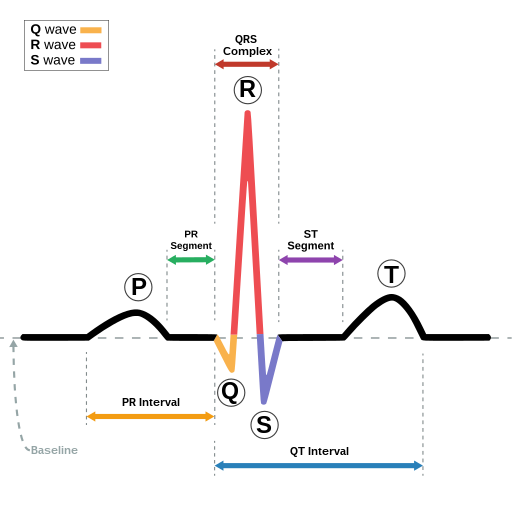
\includegraphics[width=.5\linewidth]{img/ecg-morphology.png}
  \caption{Morfologi gelombang ECG}
  Sumber: \textcite{wiki:xxx}
  \label{fig: ecg-morphology}
\end{figure}

\subsection{\textit{MIT-BIH Arrhythmia Database}}
\label{subsec: landasan-mitbih}

% \textit{MIT-BIH Arrhythmia Database} adalah dataset publik yang berisi rekaman ECG dari 47 pasien yang berdurasi 30 menit \parencite{moodyImpactMITBIHArrhythmia2001}.
\textit{MIT-BIH Arrhythmia Database} merupakan salah satu dataset publik yang dikembangkan oleh \textit{Massachusetts Institute of Technology} (MIT) dan \textit{Beth Israel Hospital} (BIH) \parencite{moodyImpactMITBIHArrhythmia2001}.
MIT-BIH Arrhythmia Database menjadi salah satu dataset standar yang banyak digunakan dalam penelitian terkait analisis sinyal ECG.
Dataset ini berisi 48 rekaman ECG dari 47 pasien yang masing-masing berdurasi 30 menit dan terdiri dari dua kanal.
Dari 48 rekaman tersebut, data 102, 104, 107, dan 217 berisi data detak jantung yang sedang dipacu.
Dataset ini direkam dengan frekuensi 360 Hz dan resolusi 11-bit.
Setiap detak jantung pada dataset, telah diberi label dan anotasi oleh para ahli.
% Pemberian label pada detak jantung dilakukan dengan menggunakan simbol-simbol tertentu.
% Simbol-simbol tersebut dideskripsikan pada tabel \ref{tab:beat_symbols}.
Pemberian label dilakukan menggunakan simbol-simbol tertentu yang dijelaskan dalam Tabel \ref{tab:beat_symbols}.

% tabel simbol yang digunakan pada dataset

% Symbol	Meaning
% · or N	Normal beat
% L	Left bundle branch block beat
% R	Right bundle branch block beat
% A	Atrial premature beat
% a	Aberrated atrial premature beat
% J	Nodal (junctional) premature beat
% S	Supraventricular premature beat
% V	Premature ventricular contraction
% F	Fusion of ventricular and normal beat
% [	Start of ventricular flutter/fibrillation
% !	Ventricular flutter wave
% ]	End of ventricular flutter/fibrillation
% e	Atrial escape beat
% j	Nodal (junctional) escape beat
% E	Ventricular escape beat
% /	Paced beat
% f	Fusion of paced and normal beat
% x	Non-conducted P-wave (blocked APB)
% Q	Unclassifiable beat
% |	Isolated QRS-like artifact

\begin{table}[H]
    \centering
    \caption{Deskripsi simbol pada \textit{MIT-BIH Arrhythmia Database}}
    \begin{tabular}{|c|l|}
    \hline
    \textbf{Simbol} & {\centering \textbf{Deskripsi}} \\
    \hline
    % $\cdot$ or N & Normal beat \\
    $\cdot$ atau N & Denyut normal \\
    % L & Left bundle branch block beat \\
    L & Denyut \textit{left bundle branch block} (LBBB) \\
    % R & Right bundle branch block beat \\
    R & Denyut \textit{right bundle branch block} (RBBB) \\
    % A & Atrial premature beat \\
    A & \textit{Atrial premature beat} (APB) \\
    % a & Aberrated atrial premature beat \\
    a & \textit{Aberrated atrial premature beat} \\
    % J & Nodal (junctional) premature beat \\
    J & \textit{Nodal (junctional) premature beat} \\
    % S & Supraventricular premature beat \\
    S & \textit{Supraventricular premature beat} \\
    % V & Premature ventricular contraction \\
    V & \textit{Premature ventricular contraction} (PVC) \\
    % F & Fusion of ventricular and normal beat \\
    F & Gabungan denyut ventrikel dan normal \\
    % {[} & Start of ventricular flutter/fibrillation \\
    {[} & Awal dari \textit{ventricular flutter/fibrillation} \\
    % ! & Ventricular flutter wave \\
    ! & \textit{Ventricular flutter wave} \\
    % {]} & End of ventricular flutter/fibrillation \\
    {]} & Akhir dari \textit{ventricular flutter/fibrillation} \\
    % e & Atrial escape beat \\
    e & \textit{Atrial escape beat} \\
    % j & Nodal (junctional) escape beat \\
    j & \textit{Nodal (junctional) escape beat} \\
    % E & Ventricular escape beat \\
    E & \textit{Ventricular escape beat} \\
    % / & Paced beat \\
    / & Denyut yang dipacu \\
    % f & Fusion of paced and normal beat \\
    f & Gabungan denyut dipacu dan normal \\
    % x & Non-conducted P-wave (blocked APB) \\
    x & Gelombang P yang tidak terkonduksi \\
    % Q & Unclassifiable beat \\
    Q & Denyut yang tidak dapat diklasifikasikan \\
    % | & Isolated QRS-like artifact \\
    \hline
    \end{tabular} \\
    \vspace{0.5em}
    Sumber: \textcite{moodyImpactMITBIHArrhythmia2001}
    \label{tab:beat_symbols}
\end{table}

\subsection{\textit{Long Short-Term Memory} (LSTM)}
\label{subsec: landasan-lstm}

\textit{Long Short-Term Memory} atau dapat disingkat LSTM merupakan pengembangan dari metode \textit{deep learning Recurrent Neural Network} (RNN). LSTM dirancang untuk mengatasi salah satu masalah yang umum terjadi pada RNN tradisional, yaitu hilangnya informasi masa lalu \parencite{hochreiterLongShorttermMemory1997}. Metode LSTM dapat diterapkan pada klasifikasi, pengolahan, dan prediksi berdasarkan data sekuensial, seperti teks dan suara,  termasuk juga data yang terkait dengan bidang kesehatan.

\begin{figure}[H]
  \centering
  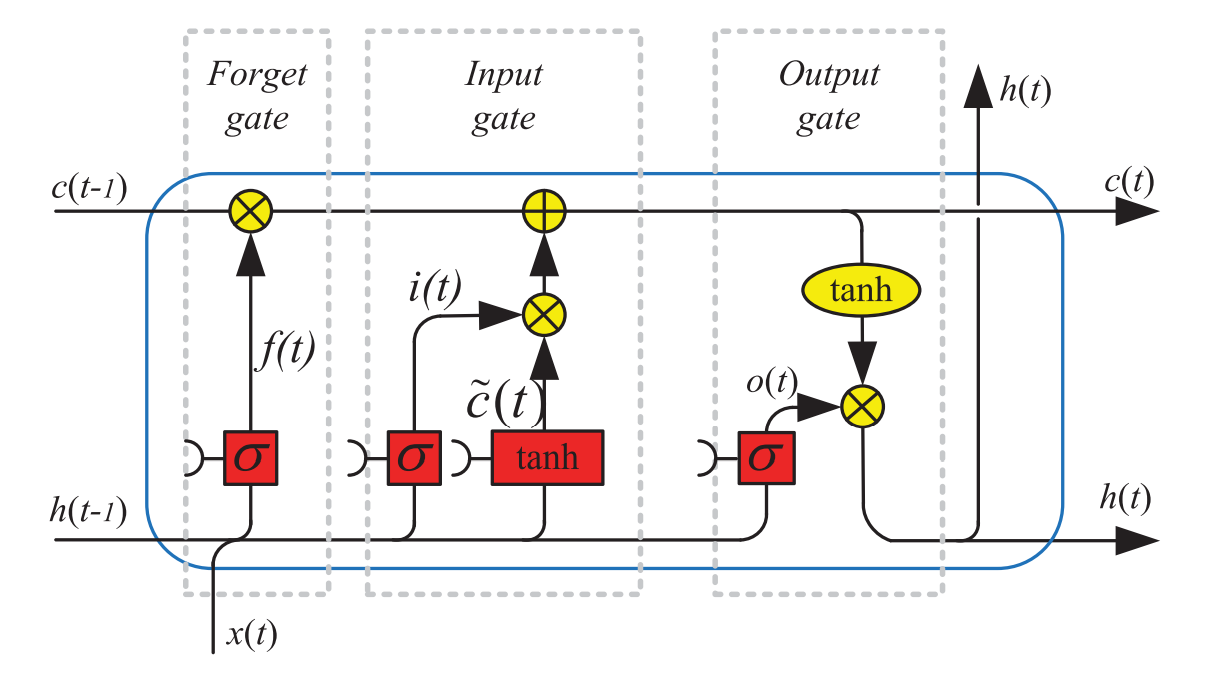
\includegraphics[width=.7\linewidth]{img/ecg-arch.png}
  \caption{Arsitektur sel LSTM}
  Sumber: \textcite{yuReviewRecurrentNeural2019}
  \label{fig:arsitektur-lstm}
\end{figure}

Gambar \ref{fig:arsitektur-lstm} menunjukkan arsitektur sel LSTM. Sebuah sel LSTM umumnya terdiri dari tiga buah \textit{gate}, yaitu \textit{input gate, output gate}, dan \textit{forget gate}. Ketiga gate tersebut berfungsi untuk mengatur informasi yang masuk maupun keluar dari sel LSTM.
\textit{Input gate} menentukan informasi baru yang akan disimpan pada \textit{cell state} (Ct), \textit{output gate} menentukan informasi apa yang akan jadi output, dan \textit{forget gate} menentukan informasi apa yang akan dibuang dari \textit{cell state} \parencite{yuReviewRecurrentNeural2019}.

Berdasarkan gambar \ref{fig:arsitektur-lstm}, secara matematis LSTM dapat didefinisikan dengan persamaan \ref{def-lstm}.
\begin{equation}
\begin{split}
    f_t &= \sigma (W_{fh}h_{t-1} + W_{fx}x_t + b_f), \\
    i_t &= \sigma (W_{ih}h_{t-1} + W_{ix}x_t + b_i),\\
    \tilde{c}_t &= \tanh (W_{\tilde{c}h}h_{t-1} + W_{\tilde{c}x}x_t + b_{\tilde{c}}), \\
    c_t &= f_t \cdot c_{t-1}+ i_t \cdot \tilde{c}_t,\\
    o_t &= \sigma (W_{oh}h_{t-1} + W_{ox}x_t + b_o), \\
    h_t &= o_t \cdot \tanh(c_t).
\end{split}
    \label{def-lstm}
\end{equation}
\noindent
Di mana \(f_t\), \(i_t\), \(o_t\) dan \(c_t\) masing-masing menunjukkan nilai \emph{forget gate}, \emph{input gate}, \emph{output gate}, dan \emph{cell state}.

% \subsection{Raspberry Pi 3}
% \label{subsec: landasan-raspi}
%
% %raspi secara umum
% Raspberry Pi merupakan sebuah komputer mini seukuran kartu kredit yang dikembangkan oleh Raspberry Pi Foundation \parencite{8756967}. 
% Raspberry Pi memiliki beberapa kelebihan, seperti ukurannya yang kecil, konsumsi daya yang rendah, harga yang terjangkau, serta kemampuan komputasi baik.
% %need citation
% Raspberry Pi dapat diaplikasikan pada berbagai bidang, seperti industri, agrikultur, bioteknologi, dan kesehatan \parencite{9760691}.
%
% %raspi 4 
% %*sekara sudah bukan yang terbaru, sudah ada raspi 5
% % Raspberry Pi 4 model B merupakan salah satu varian dari Raspberry Pi generasi keempat. Raspberry Pi 4 model B memiliki spesifikasi prosesor \textit{quad-core} ARM Cortex-A72 1.5GHz, dengan pilihan RAM 2GB, 4GB, atau 8GB LPDDR4-3200 SDRAM. Raspberry Pi 4 model B juga dilengkapi dengan konektivitas WiFi 2.4GHz dan 5GHz, Bluetooth 5.0, serta \textit{ethernet} dengan kecepatan maksimum 1Gbps. Raspberry Pi 4 model B juga memiliki \textit{port micro} HDMI, USB 3.0, USB 2.0, dan port GPIO.
%
% % raspi 3
% % Pengujian dilakukan pada perangkat Raspberry Pi 3B. Perangkat ini memiliki prosesor ARMv8 quad-core 1,2GHz dan RAM 1GB LPDDR2. Konektivitas perangkat ini didukung dengan 2.4Ghz WiFi serta \textit{ethernet} dengan kecepatan maksimum 100Mbps.
% Raspberry Pi 3 merupakan salah satu varian dari Raspberry Pi generasi ketiga. Raspberry Pi 3 memiliki spesifikasi prosesor ARMv8 \textit{quad-core} 1,2GHz dan RAM 1GB LPDDR2. Raspberry Pi 3 juga telah dilengkapi dengan konektivitas WiFi 2.4GHz dan \textit{ethernet} dengan kecepatan maksimum 100Mbps. Raspberry Pi 3 juga memiliki \textit{port} HDMI, USB 2.0, dan \textit{port} GPIO.

% klasifikasi detak jantung
% tentang detak jantung menurut AAMI

% heart related disease class
% N, sveb, veb, f, dan q
% \section{Klasifikasi Detak Jantung}

% \section{Inferensi}

% metrik evaluasi
% akurasi, presisi, recall, f1-score

% TODO
% landasan teori lain
% penerapan lstm di edge device


%%%%%%%%%%%%%%%%%%%%%%%%%%%%%%%%%%%%%%%%%%%%%%%%%%%%%%%%%%%%%%%%%%%%%%%
% BAB 3
%%%%%%%%%%%%%%%%%%%%%%%%%%%%%%%%%%%%%%%%%%%%%%%%%%%%%%%%%%%%%%%%%%%%%%%

% studi literatur
% pembuatan model classifier
% implementasi inferenciing
% pengujian
% pembahasan

% TO DO: Parameter uji

\mychapter{3}{BAB 3 METODOLOGI}

% TO DO: alur penelitian
% studi literatur, pembuatan model, implementasi dan pengujian, penarikan kesimpulan
Penelitian ini dilakukan dengan beberapa tahapan, yaitu studi literatur, pembuatan model, implementasi, pengujian, dan penarikan kesimpulan. Gambar \ref{fig:alur-penelitian} menunjukkan alur penelitian yang digunakan pada penelitian ini.

\begin{figure}[tph]
	\centering
	\includegraphics[width=.45\linewidth]{./img/lstm-alur penelitian.drawio.pdf}
	\caption{Alur penelitian}
	\label{fig:alur-penelitian}
\end{figure}

\section{Studi Literatur}
\label{subsec: metodologi-studi-literatur}
% - Tujuan studi literatur
% - Metode studi literatur: 

Studi literatur dilakukan untuk memperdalam pengetahuan penulis terkait implementasi model LSTM untuk klasifikasi detak jantung.
% Studi literatur dilakukan dengan cara mencari dasar teori terkait dengan implementasi model LSTM pada klasifikasi detak jantung, serta melakukan \textit{review} terhadap penelitian-penelitian terdahulu yang berkaitan dengan klasifikasi detak jantung menggunakan sinyal ECG.
% Studi literatur dilakukan dengan mencari dasar teori dan melakukan \textit{review} terhadap penelitian-penelitian terdahulu yang berkaitan dengan klasifikasi detak jantung menggunakan sinyal ECG.
Studi literatur ini dilakukan dengan cara meninjau beberapa penelitian terdahulu dan mencari dasar teori yang berkaitan dengan implementasi model LSTM untuk klasifikasi detak jantung.
Sumber literatur yang digunakan dalam penelitian ini meliputi jurnal ilmiah, konferensi, serta dokumentasi resmi.
Dasar teori yang relevan dengan penelitian ini berkaitan dengan detak jantung, sinyal ECG, dan model LSTM.
Dasar teori tersebut antara lain:
\begin{enumerate}
	\item Detak jantung

		Dasar teori mengenai detak jantung diperlukan untuk memahami karakteristik detak jantung normal dan abnormal, serta faktor-faktor yang mempengaruhi detak jantung.
		Informasi ini penting untuk memastikan bahwa model klasifikasi yang dikembangkan mampu membedakan dengan tepat antara berbagai jenis detak jantung.
		
	\item Sinyal ECG

		Studi literatur mengenai sinyal ECG diperlukan untuk memahami apa itu sinyal ECG dan bagaimana sinyal ECG dapat digunakan dalam klasifikasi detak jantung.
		Hal-hal yang perlu dipahami antara lain karakteristik sinyal ECG, proses perekaman sinyal ECG, serta bagaimana sinyal ECG dapat digunakan dalam klasifikasi detak jantung.

	\item Model LSTM

		Dasar teori dari LSTM diperlukan untuk mendapatkan pemahaman komprehensif terkait dengan model LSTM.
		Dari studi literatur terkait LSTM ini, akan didapatkan informasi mengenai karakteristik LSTM, cara kerja LSTM, serta bagaimana LSTM dapat diterapkan dalam analisis data time-series.
		Informasi ini akan menjadi acuan untuk mengimplementasikan LSTM dalam klasifikasi detak jantung.

\end{enumerate}



% Pada tahap ini, dilakukan studi literatur dengan cara melakukan \textit{review}
% terhadap penelitian-penelitian terdahulu yang berkaitan dengan klasifikasi detak jantung menggunakan ECG
% untuk mengetahui \textit{state-of-the-art} dari penelitian terkait.
% Pada tahap ini juga dilakukan pencarian referensi terkait dengan klasifikasi detak jantung,
% sinyal ECG, dan model LSTM yang akan digunakan pada penelitian ini untuk memperdalam pengetahuan penulis.
% Sumber utama yang digunakan adalah jurnal ilmiah, konferensi, serta dokumentasi resmi.


% \section{Pengumpulan Data}
% \label{subsec: metodologi-pengumpulan-data}
%
% Data yang digunakan untuk melakukan pelatihan pada penelitian ini diperoleh dari dataset publik \textit{MIT‐BIH arrhythmia database} \parencite{moodyImpactMITBIHArrhythmia2001}.
% Dataset dapat diakses melalui tautan \url{https://physionet.org/content/mitdb/1.0.0/}.
% Dataset tersebut terdiri atas 48 data rekaman yang diambil dari 47 pasien.
% Setiap detak jantung pada dataset tersebut telah diberi label dan anotasi oleh para ahli.
% Pada dataset tersebut, data 102, 104, 107, dan 217 berisi data detak jantung yang sedang dipacu, sehingga tidak digunakan pada penelitian ini.
% Setiap rekaman memiliki durasi 30 menit dan terdiri dari dua kanal.
% Pada penelitian ini, hanya satu kanal yang digunakan, yaitu kanal \textit{Modified Lead II}.
% % Anotasi tersebut dapat dipetakan menjadi kelas sesuai dengan kelas rekomendasi AAMI, yaitu N, SVEB, VEB, F, dan Q \parencite{associationfortheadvancementofmedicalinstrumentationTestingReportingPerformance1998}. Pemetaan tersebut dapat dilihat pada Tabel \ref{tab:aami-label}.
%
% % Ini tidak dibahas detail
% % cukup penjelasan narasi singkat
% % TO DO: pindah ke bab 2
%
% % \begin{table}[h]
% % 	\caption{Kelas Rekomendasi AAMI dan Label pada MIT-BIH}
% % 	\begin{center}
% % 		\begin{tabular}{c @{\hspace{1cm}} c}
% % 			\hline
% % 			AAMI                              & MIT-BIH       \\
% % 			\hline
% % 			Normal (N)                        & N, L, R, e, j \\
% % 			Supraventricular Ectopic Beat (S) & A, a, J, S    \\
% % 			Ventricular Ectopic Beat (V)      & V, E          \\
% % 			Fusion (F)                        & F             \\
% % 			Unknown (Q)                       & /, f, Q       \\
% % 			\hline
% % 		\end{tabular}
% % 	\end{center}
% % 	\label{tab:aami-label}
% % \end{table}

% \section{Pembuatan Model}
\section{Perancangan Model}
\label{subsec: metodologi-pembuatan-model}
Pada tahap ini, dilakukan perancangan model yang akan digunakan untuk melakukan klasifikasi detak jantung.
Model dirancang untuk dapat melakukan klasifikasi detak jantung menjadi 5 kelas, yaitu Normal (N), \textit{Supraventricular Ectopic Beat} (S), \textit{Ventricular Ectopic Beat} (V), \textit{Fusion} (F), dan \textit{Unknown} (Q) sesuai dengan rekomendasi AAMI \parencite{associationfortheadvancementofmedicalinstrumentationTestingReportingPerformance1998}.
Terdapat tiga jenis model yang akan digunakan pada penelitian ini, yaitu LSTM, Bi-LSTM, dan LSTM-FCN.
LSTM dan Bi-LSTM merupakan varian dari Recurrent Neural Network (RNN) yang mampu menangani data \textit{time-series} seperti sinyal ECG, sedangkan LSTM-FCN menggabungkan LSTM dengan Convolutional Neural Network (CNN) 
% untuk menangkap fitur temporal dan spasial secara lebih efektif.
untuk dapat mengekstraksi fitur dengan lebih baik.
% Pada versi original, untuk menghindari \textit{overfitting}, terdapat \textit{dimension shuffle} yang akan mengacak input sebelum blok LSTM. Akan tetapi, meletakkan \textit{dimension shuffle} sebelum blok LSTM akan menyebabkan hilangnya informasi pada dimensi waktu \parencite{8713870}. Pada penelitian ini kami melakukan modifikasi pada LSTM-FCN dengan menukar posisi \textit{dimension shuffle} pada sebelum blok \textit{convolutional}.

Pada model LSTM-FCN terdapat \textit{layer dimension shuffle} yang digunakan untuk mengurangi \textit{overfitting}.
Akan tetapi, meletakkan \textit{layer dimension shuffle} sebelum blok LSTM akan menyebabkan hilangnya informasi pada dimensi waktu \parencite{8713870}.
Oleh karena itu, pada penelitian ini dilakukan modifikasi pada LSTM-FCN dengan menukar posisi \textit{layer dimension shuffle} pada sebelum blok \textit{convolutional}.
% Pembuatan model meliputi \textit{preprocessing} data, ekstraksi fitur, pelatihan model, dan evaluasi model.

\section{Pelatihan Model}
\label{subsec: metodologi-pelatihan-model}
% - Parameter pelatihan
% - Metode pelatihan
Pada tahap ini, dilakukan pelatihan model LSTM, Bi-LSTM, dan LSTM-FCN menggunakan data ECG yang telah diproses.
Pelatihan model dilakukan dengan menggunakan bantuan \textit{framework} TensorFlow.
Sebelum dilakukan pelatihan, data ECG yang digunakan akan dipisahkan menjadi data latih dan data uji dengan perbandingan 70:30.
Pemisahan data ini dilakukan untuk memastikan bahwa model yang dibuat mampu menggeneralisasi data dengan baik.

% Proses pelatihan mencakup beberapa langkah utama, yaitu normalisasi data, pembentukan batch, dan optimasi hiperparameter.
% Model dilatih menggunakan algoritma optimasi seperti Adam dengan berbagai konfigurasi laju pembelajaran.
Selama proses pelatihan, terdapat beberapa hiperparameter yang perlu diatur, seperti jumlah \textit{epoch}, ukuran \textit{batch}, dan \textit{learning rate}.
%tidak ada optimasi hiperparameter, hiperparameter sudah ditentukan di awal
Hiperparameter yang digunakan antara lain jumlah \textit{epoch} sebanyak 50, ukuran \textit{batch} 256, dan \textit{learning rate} sebesar 0.001.
Evaluasi performa model dilakukan menggunakan metrik akurasi, presisi, recall, dan F1-score untuk setiap model.
% Hasil evaluasi ini kemudian dianalisis untuk menentukan model yang paling baik untuk klasifikasi detak jantung.

% \section{Evaluasi Model}
% \label{subsec: metodologi-evaluasi-model}
% - Metode evaluasi
% - Metrik evaluasi

\section{Implementasi dan Pengujian Inferensi}
\label{subsec: metodologi-implementasi}

Untuk melakukan inferensi model, diperlukan implementasi model pada perangkat yang akan digunakan.
% Implementasi dilakukan dengan membuat aplikasi berbasis web yang dibuat dengan menggunakan menggunakan bahasa pemrograman Python dan \textit{framework} Flask.
Model diimplementasikan dalam bentuk aplikasi berbasis web.
% Aplikasi ini digunakan untuk melakukan inferensi pada data detak jantung yang diperoleh dari sensor ECG.
Aplikasi akan menerima data ECG dan akan mengembalikan keluaran berupa hasil klasifikasi detak jantung.
Nantinya, aplikasi ini akan diaplikasikan pada perangkat Raspberry Pi 4 dan Intel NUC.

% ini pindah ke bab 5 (implementasi dan pengujian)
% Sebelum diimplementasikan, model dioptimasi terlebih dahulu agar dapat beroperasi secara efisien terutama pada perangkat dengan daya komputasi rendah seperti Raspberry Pi.
% Model dioptimasi dengan cara melakukan konversi ke dalam bentuk TensorFlow Lite (tflite).
% Model TensorFlow Lite memiliki ukuran yang lebih kecil dan membutuhkan lebih sedikit dependensi dibanding dengan model TensorFlow.
% Pada proses optimasi, juga dilakukan kuantisasi yang dapat mengurangi penggunaan memori dan mempercepat komputasi
% sehingga cocok untuk perangkat dengan spesifikasi rendah seperti Raspberry Pi.

% flowchart aplikasi

% \section{Pengujian}
% \label{subsec: metodologi-pengujian}

% Pengujian dilakukan pada perangkat Raspberry Pi 3B. Perangkat ini memiliki prosesor ARMv8 quad-core 1,2GHz dan RAM 1GB LPDDR2. Konektivitas perangkat ini didukung dengan 2.4Ghz WiFi serta \textit{ethernet} dengan kecepatan maksimum 100Mbps.
% pindah ke landasan teori

Pada tahap pengujian, dilakukan pengujian inferensi model pada perangkat Raspberry Pi 4 dan Intel NUC.
Tujuan dari pengujian ini adalah untuk mengevaluasi performa inferensi dari model yang telah dibuat pada beberapa perangkat.
Pengujian dilakukan menggunakan data uji berupa data ECG yang diperoleh dari sensor ECG Polar H10.
Metrik pengujian yang digunakan adalah waktu prediksi dan penggunaan memori saat melakukan inferensi pada perangkat.
Data detak jantung yang digunakan dalam pengujian memiliki durasi sepanjang 10 detik, 1 menit, dan 10 menit.
Pengujian dilakukan menggunakan tiga model yang telah dilatih sebelumnya, yaitu LSTM, Bi-LSTM, dan LSTM-FCN.
Setiap pengujian diulang sebanyak 5 kali untuk setiap jenis model, dan hasil yang diperoleh kemudian dijadikan nilai rata-rata sebagai hasil akhir.

\section{Penarikan Kesimpulan}
\label{subsec: metodologi-penarikan-kesimpulan}
Penarikan kesimpulan dilakukan setelah melakukan seluruh tahapan penelitian mulai, dari studi literatur hingga pengujian.
Kesimpulan tersebut didasarkan pada hasil pengujian dan analisis yang telah dilakukan.
Kesimpulan yang diperoleh diharapkan dapat menjawab rumusan masalah yang telah diajukan dalam penelitian ini.

% \section{Pembahasan}
% \label{subsec: metodologi-pembahasan}
%
% Pada tahap ini, hasil pengujian akan dianalisis secara mendalam.
% Hasil pengujian model akan dibandingkan untuk mencari model dengan performa terbaik.
% Selain itu, hasil pengujian juga akan dibandingkan dengan hasil penelitian-penelitian sebelumnya.
% % Hasil dari pengujian ini akan menjadi subjek utama pembahasan.

% \section{Jadwal penelitian}
% \label{subsec:label}
%
% \begin{figure}[tph]
% %   \centering
% %   \includegraphics[width=.7\linewidth]{img/jadwal.png}
% %   \caption{Jadwal Penelitian}
% %   \label{fig:jadwal-penelitian}
% \end{figure}

% %%%%%%%%%%%%%%%%%%%%%%%%%%%%%%%%%%%%%%%%%%%%%%%%%%%%%%%%%%%%%%%%%%%%%%%
% BAB 4
%%%%%%%%%%%%%%%%%%%%%%%%%%%%%%%%%%%%%%%%%%%%%%%%%%%%%%%%%%%%%%%%%%%%%%%




% question: perancangan model? atau digabung dengan tahap pelatihan model?


\mychapter{4}{BAB 4 PERANCANGAN SISTEM}

Pada bab ini, akan dijelaskan tahap-tahap yang dilakukan dalam perancangan sistem klasifikasi detak jantung yang digunakan dalam penelitian ini.
Perancangan sistem meliputi tahap \textit{preprocessing} data, ekstraksi fitur, perancangan model LSTM, pelatihan model, dan evaluasi model.
Gambar \ref{fig:alur-sistem} menunjukkan alur perancangan sistem yang digunakan dalam penelitian ini.

%
\begin{figure}[H]
  \begin{center}
    \includegraphics[width=1\textwidth]{img/lstm-ML Pipeline.drawio.pdf}
  \end{center}
  \caption{Alur perancangan sistem}
  \label{fig:alur-sistem}
\end{figure}

\section{\emph{Preprocessing} Data}
\label{subsec: bab4-preprocessing-data}
 
Dataset yang digunakan dalam penelitian ini diperoleh dari MIT-BIH Arrhythmia Database.
% Sebelum data dapat digunakan untuk pelatihan model, data ECG harus melalui tahap \textit{preprocessing}.
% \textit{Preprocessing} dilakukan untuk memastikan kualitas dan keandalan data yang digunakan dalam proses pelatihan model. 
% Terdapat beberapa tahap \textit{preprocessing} yang dilakukan pada penelitian ini, yaitu pemetaan dataset, penghapusan \textit{noise} berfrekuensi tinggi, penghapusan \textit{baseline wander} (BW), dan normalisasi.
Data ECG pada MIT-BIH Arrhythmia Database memiliki anotasi yang terdiri dari 20 kelas, sedangkan pada penelitian ini hanya menggunakan 5 kelas, yaitu Normal (N), \textit{Supraventricular Ectopic Beat} (S), \textit{Ventricular Ectopic Beat} (V), \textit{Fusion} (F), dan \textit{Unknown} (Q).
Kelas-kelas tersebut dipilih berdasarkan rekomendasi dari Association for the Advancement of Medical Instrumentation (AAMI), yang mengelompokkan berbagai jenis aritmia ke dalam kategori yang lebih umum.
Oleh karena itu, perlu dilakukan pemetaan kelas pada dataset agar sesuai dengan kelas yang digunakan pada penelitian ini.
Pemetaan tersebut dapat dilihat pada Tabel \ref{tab:aami-label}, yang menunjukkan bagaimana kelas-kelas dari dataset dipetakan ke dalam 5 kelas yang digunakan dalam penelitian ini.

\begin{table}[h]
	\caption{Kelas rekomendasi AAMI dan simbol pada MIT-BIH}
	\begin{center}
		\begin{tabular}{|l @{\hspace{1cm}} |l|}
			\hline
			% \textbf{AAMI}                              & \textbf{MIT-BIH}       \\
			\multicolumn{1}{|c|}{\textbf{AAMI}} & \multicolumn{1}{c|}{\textbf{MIT-BIH}} \\
			\hline
			Normal (N)                        & N, L, R, e, j \\
			\hline
                        \textit{Supraventricular Ectopic Beat} (S) & A, a, J, S    \\
			\hline
                        \textit{Ventricular Ectopic Beat} (V)      & V, E          \\
			\hline
                        \textit{Fusion} (F)                        & F             \\
			\hline
                        \textit{Unknown} (Q)                       & /, f, Q       \\
			\hline
		\end{tabular}
	\end{center}
	\label{tab:aami-label}
\end{table}

% table count
% 0    86399
% 2     6512
% 1     2692
% 3      787
% 4        8

Jumlah data pada setiap kelas setelah dilakukan pemetaan dapat dilihat pada Tabel \ref{tab:count-label}.
Jumlah seluruh detak jantung pada dataset yang digunakan dalam penelitian ini adalah 96398 detak.
Dari tabel tersebut dapat dilihat bahwa kelas Normal (N) memiliki jumlah data terbanyak dengan jumlah 86399 data.
Sementara itu, kelas \textit{Unknown} (Q) memiliki jumlah data terendah dengan jumlah 8 data.
% Terdapat ketidakseimbangan kelas yang cukup signifikan pada dataset, dengan kelas minoritas yang memiliki jumlah kurang dari 1\% dari kelas mayoritas.
Terdapat ketidakseimbangan kelas yang cukup signifikan pada dataset.
Kelas minoritas, yaitu \textit{Unknown} (Q), memiliki jumlah data kurang dari 1\% dari kelas mayoritas.


\begin{table}[H]
  \caption{Jumlah data pada setiap kelas}
  \begin{center}
    \begin{tabular}{|l @{\hspace{1cm}} |c|}
      \hline
      % \textbf{Kelas} & \textbf{Jumlah Data} \\
      \multicolumn{1}{|c|}{\textbf{Kelas}} & \multicolumn{1}{c|}{\textbf{Jumlah Data}} \\
      \hline
      Normal (N)                        & 86399 \\
      \hline
      \textit{Supraventricular Ectopic Beat} (S) & 2692  \\
      \hline
      \textit{Ventricular Ectopic Beat} (V)      & 6512  \\
      \hline
      \textit{Fusion} (F)                        & 787   \\
      \hline
      \textit{Unknown} (Q)                       & 8     \\
      \hline
      % \textbf{Jumlah Total} & 96398 \\
      \multicolumn{1}{|c|}{\textbf{Jumlah Total}} & \multicolumn{1}{c|}{96398} \\
      \hline
    \end{tabular}
  \end{center}
  \label{tab:count-label}
\end{table}

% % metode penghilangan frekuensi tinggi
% %     ecg = denoise_wavelet(ecg, method='VisuShrink', mode='soft', wavelet_levels=10, wavelet='db8', rescale_sigma='True')
%
% Selama proses pengambilan data, sinyal ECG rentan terhadap \textit{noise} berfrekuensi tinggi.
% Frekuensi tinggi pada data ECG dianggap sebagai \textit{noise} yang dapat mengganggu proses klasifikasi detak jantung, sehingga perlu dilakukan penghilangan \textit{noise} tersebut.
% Pada penelitian ini, \textit{noise} berfrekuensi tinggi dihilangkan dengan menggunakan metode \textit{wavelet denoise}.
% \textit{Wavelet denoise} merupakan metode yang digunakan untuk menghilangkan \textit{noise} pada sinyal maupun gambar dengan menggunakan \textit{wavelet transform}.
% \textit{Wavelet transform} memungkinkan sinyal untuk dipecah menjadi beberapa bagian frekuensi yang berbeda, sehingga memungkinkan penghilangan \textit{noise} pada frekuensi tertentu.
% Metode \textit{wavelet denoise} yang digunakan pada penelitian ini adalah \textit{VisuShrink} dengan mode \textit{soft thresholding}, dan menggunakan \textit{wavelet} Daubechies 8 (db8) dengan 10 level \textit{wavelet decomposition}.
%
% % --- dijelaskan lebih detail? ---
%
% % Sinyal ECG diubah ke dalam domain \textit{wavelet} dengan menggunakan \textit{wavelet transform} Daubechies 8 (db8) dengan 10 level \textit{wavelet decomposition}.
% % \textit{Noise} pada sinyal ECG kemudian dapat dihilangkan dengan mengurangi koefisien \textit{wavelet} yang memiliki nilai di bawah ambang batas tertentu.
%
% %
% % Setelah menghilangkan \textit{noise} berfrekuensi tinggi, tahap selanjutnya adalah menghilangkan \textit{baseline wander} (BW).
% % elaborate
% Selain \textit{noise} berfrekuensi tinggi, sinyal ECG juga rentan terhadap \textit{baseline wander}.
% \textit{Baseline wander} (BW) merupakan \textit{noise} berfrekuensi rendah yang terdapat pada ECG.
% BW dapat disebabkan oleh beberapa faktor, seperti pernapasan, elektroda yang bermuatan listrik, dan gerakan dari pasien \parencite{lenisComparisonBaselineWander2017}.
% % metode baseline wander
%         % baseline = medfilt(ecg, 71)
%         % baseline = medfilt(baseline, 215)
%         %
%         % # Remove Baseline
%         % for i in range(0, len(ecg)):
%         %     ecg[i] = ecg[i] - baseline[i]
% % BW dihilangkan dengan menggunakan metode \textit{median filter} dengan panjang jendela 71 dan 215.
% BW dihilangkan dengan melakukan substraksi antara sinyal ECG dengan \textit{trend} sinyal.
% \textit{Trend} sinyal diperoleh dengan menggunakan metode \textit{median filter} sebanyak dua kali dengan panjang jendela 71 dan 215.
% % Median filtering, as mentioned earlier, is another method commonly used for baseline wander removal. It involves replacing each data point in the signal with the median value within a specified window around that point. This approach can effectively remove baseline variations while preserving the shape of the ECG waveform.
% \textit{Median filter} akan menggantikan setiap titik data pada sinyal dengan nilai median dalam jendela yang ditentukan.
% \textit{Median filter} didefinisikan oleh persamaan \ref{eq:median-filter}
% \begin{equation}
%     % perlu dicek lagi
%     y[n] = \text{median}(x[n - \frac{M}{2} : n + \frac{M}{2}])
%     \label{eq:median-filter}
% \end{equation}
% dengan $y[n]$ adalah sinyal hasil \textit{median filter}, $x[n]$ adalah sinyal asli, dan $M$ adalah panjang jendela \textit{median filter}.
% % Yang mana $y[n]$, $x[n]$, dan $M$ masing-masing menunjukkan sinyal hasil \textit{median filter}, sinyal asli, dan panjang jendela \textit{median filter}.
%
% % Setelah \textit{baseline wander} dihilangkan, data dinormalisasi untuk menghindari perbedaan skala.
% % Setelah \textit{nose} dan \textit{baseline wander} dihilangkan, data dinormalisasi untuk menghindari perbedaan skala.
% % Normalisasi yang dilakukan yaitu \textit{Z-score normalization}.
% % metode normalisasi
% Setelah \textit{noise} dan \textit{baseline wander} dihilangkan, tahap selanjutnya adalah normalisasi data.
% Normalisasi dilakukan untuk menghindari adanya perbedaan skala pada data.
% Metode normalisasi yang digunakan pada penelitian ini adalah \textit{Z-score normalization}.
% \textit{Z-score normalization} mengubah data ke dalam distribusi normal dengan rata-rata 0 dan standar deviasi 1.
% \textit{Z-score normalization} didefinisikan oleh persamaan \ref{eq:z-score}
% \begin{equation}
% 		z = \frac{x - \mu}{\sigma}
% 		\label{eq:z-score}
% \end{equation}
% dengan $z$ adalah data yang telah dinormalisasi, $x$ adalah data asli, $\mu$ adalah rata-rata data, dan $\sigma$ adalah standar deviasi data.
%
%
% % Gambar \ref{fig:sebelum-prep} menunjukkan data sebelum dilakukan \textit{preprocessing}, sedangkan Gambar \ref{fig:setelah-prep} menunjukkan data setelah dilakukan \textit{preprocressing}.
% Gambar \ref{fig:sebelum-prep} dan \ref{fig:setelah-prep} memperlihatkan perbandingan data ECG sebelum dan setelah dilakukan \textit{preprocessing}.
% % Pada Gambar \ref{fig:sebelum-prep}, terlihat bahwa terdapat \textit{noise} berfrekuensi tinggi dan variasi pada \textit{baseline} sinyal ECG.
% Pada Gambar \ref{fig:sebelum-prep}, terlihat bahwa pada data ECG masih terdapat gangguan seperti \textit{noise} berfrekuensi tinggi dan variasi pada \textit{baseline} sinyal.
% % Setelah dilakukan \textit{preprocessing}, sinyal ECG menjadi lebih halus dan memiliki baseline yang lebih rata.
% Setelah dilakukan \textit{preprocessing}, sinyal ECG menjadi lebih halus dan memiliki \textit{baseline} yang lebih rata, seperti yang terlihat pada Gambar \ref{fig:setelah-prep}.
%
% \begin{figure}[H]
%     \centering
%     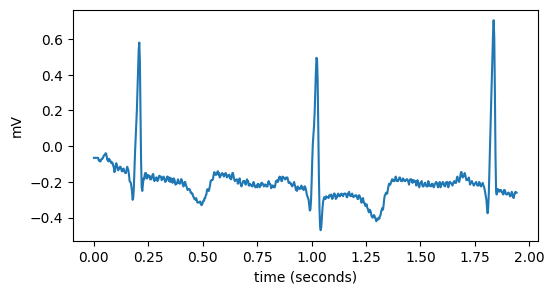
\includegraphics[width=0.6\linewidth]{./img/sebelum_prep.png}
% 	\caption{Data sebelum \textit{preprocessing}}
% 	\label{fig:sebelum-prep}
% \end{figure}
%
% \begin{figure}[H]
%   \centering
%   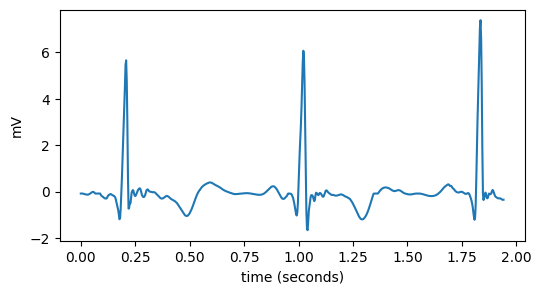
\includegraphics[width=0.6\linewidth]{./img/setelah_prep.png}
%   \caption{Data setelah \textit{preprocessing}}
%   \label{fig:setelah-prep}
% \end{figure}
%

\section{Ekstraksi Fitur}
\label{subsec: bab4-ekstraksi-fitur}

% Kami menggunakan RR-Interval sebagai fitur dalam penelitian ini.
% taruh sini atau bab 2?
% RR-Interval adalah jarak antara dua titik R pada sinyal ECG, yang merepresentasikan interval antara dua detak jantung.
% Visualisasi dari RR-Interval ditunjukkan oleh Gambar \ref{fig:rri}.
% Dalam gambar tersebut, terdapat puncak 'R' yang menandakan titik maksimum voltase selama siklus detak jantung pada sinyal ECG.
% Jarak antara dua puncak 'R' ini menunjukkan RR-Interval yang menjadi fitur utama dalam penelitian ini.
% \begin{figure}[H]
%   \centering
%   \includegraphics[scale=.7]{img/lstm-Page-7.drawio.pdf}
%   \caption{RR-Interval}
%   \label{fig:rri}
% \end{figure}

% --- pindah ke bab 2? ---

Fitur utama yang digunakan dalam penelitian ini adalah RR-Interval.
Pada dataset MIT-BIH Arrhythmia Database, sudah terdapat anotasi R-peak yang menunjukkan posisi puncak 'R' pada sinyal ECG.
Dari posisi R-peak tersebut, dapat dihitung jarak antara dua puncak 'R' untuk mendapatkan RR-Interval.
RR-Interval dihitung dengan menggunakan persamaan \ref{eq:rr-interval}
% RRi[i] = Rpeak[i+1] - Rpeak[i]
\begin{equation}
		RRi[i] = Rpeak[i+1] - Rpeak[i]
		\label{eq:rr-interval}
\end{equation}
dengan $RRi[i]$ adalah RR-Interval ke-$i$, dan $Rpeak[i]$ adalah posisi R-peak ke-$i$.
RR-Interval tersebut kemudian diekstraksi menjadi 9 fitur, yaitu RR0, RR-1, RR+1, RR0/avgRR, tRR0, RR-1/avgRR, RR-1/RR0, RR+1/avgRR, dan RR+1/RR0 \parencite{pramukantoroHeartbeatClassifierContinuous2022}.
Tabel \ref{tab:rri} menunjukkan deskripsi lengkap dari setiap fitur yang digunakan dalam penelitian ini.
Ekstraksi dilakukan dengan menggunakan jendela sepanjang 42 data. 
        % avgRR = np.mean(rr_intervals[i-42:i+1])
        % stddevRR = np.std(rr_intervals[i-42:i+1])
% Rata-rata RR-Interval (avgRR) merupakan rata-rata dari 42 data, termasuk RR-0. 
Rata-rata RR-Interval (avgRR) dan standar deviasi RR-Interval (stddevRR) dihitung dengan menggunakan persamaan \ref{eq:avg-rr} dan \ref{eq:stddev-rr}.
\begin{equation}
		\text{avgRR} = \frac{1}{42} \sum_{i=0}^{42} RRi[i]
		\label{eq:avg-rr}
\end{equation}
\begin{equation}
		\text{stddevRR} = \sqrt{\frac{1}{42} \sum_{i=0}^{42} (RRi[i] - \text{avgRR})^2}
		\label{eq:stddev-rr}
\end{equation}


\begin{table}[H]
  \caption{Deskripsi RR-Interval}
\begin{center}
\footnotesize
\begin{tabular}{|l @{\hspace{1cm}} |l|}
\hline
% \textbf{Fitur} & \textbf{Deskripsi}\\
\multicolumn{1}{|c|}{\textbf{Fitur}} & \multicolumn{1}{c|}{\textbf{Deskripsi}}\\
\hline
RR0 & Nilai RRi saat ini\\
\hline
RR-1 & Nilai RRi sebelumnya\\
\hline
RR+1  & Nilai RRi selanjutnya\\
\hline
RR0/avgRR & Nilai RRi saat ini dibagi dengan rata-rata 42 RRi sebelumnya\\
\hline
tRR0  & (RRi saat ini - rata-rata RRi) / stddevRRi\\
\hline
RR-1/avgRR & Nilai RRi sebelumnya / rata-rata RRi\\
\hline
RR-1/RR0 & Nilai RRi sebelumnya / RRi saat ini\\
\hline
RR+1/avgRR & Nilai RRi selanjutnya / rata-rata RRi\\
\hline
RR+1/RR0 & Nilai RRi selanjutnya / RRi saat ini\\
\hline
\end{tabular}
\end{center}
\center
Sumber: \textcite{pramukantoroHeartbeatClassifierContinuous2022}
\label{tab:rri}
\end{table}

%contoh extracted feature

% considering cuma pakai lstm256 tapi dengan fitur lain
\section{Perancangan Model LSTM}
\label{subsec: bab4-pembuatan-model-lstm}
% Pada tahap ini, penulis membuat model berbasis LSTM yang akan digunakan untuk melakukan klasifikasi detak jantung. 
% Dalam penelitian ini, 
% Pembuatan model meliputi pembuatan arsitektur model, pelatihan model, dan evaluasi model.
% Model dibuat dengan menggunakan \textit{framework} TensorFlow dan dilatih sebanyak 50 \textit{epoch}.


% LSTM merupakan pengembangan dari \textit{Recurrent Neural Network} (RNN) yang dirancang untuk mengatasi masalah yang umum terjadi pada RNN tradisional, yaitu hilangnya informasi masa lalu \parencite{hochreiterLongShorttermMemory1997}.  LSTM memiliki kemampuan untuk mengingat informasi yang disimpan dalam jangka waktu yang lama. 


Terdapat tiga jenis model yang akan digunakan pada penelitian, yaitu \textit{Long Short-Term Memory} (LSTM), \textit{Bidirectional} LSTM (Bi-LSTM), serta LSTM \textit{Fully Convolutional Network} (LSTM-FCN). 
Arsitektur model LSTM yang digunakan dalam penelitian ini ditunjukkan oleh Gambar \ref{fig:arslstm}. Model terdiri dari tiga \textit{layer}, yakni satu buah LSTM \textit{layer} dan dua buah \textit{dense layer}. 
% Terdapat dua varian model LSTM yang dilatih dengan menggunakan dua \textit{hyperparameter} berbeda.
% Terdapat dua varian model LSTM dengan menggunakan dua \textit{hyperparameter} berbeda.
Dalam penelitian ini, digunakan dua model LSTM dengan \textit{hyperparameter} yang berbeda.
Model pertama memiliki 512 unit LSTM pada \textit{layer} pertama dan 256 unit \textit{dense} pada \textit{layer} kedua. Sementara itu, model kedua memiliki 256 unit LSTM pada layer pertama dan 128 unit \textit{dense} pada \textit{layer} kedua.

% img arsi lstm
\begin{figure}[H]
  \centering
  \includegraphics[scale=.9, angle=-90]{img/lstm-Page-2.drawio.pdf}
  \caption{Arsitektur LSTM}
  \label{fig:arslstm}
\end{figure}

\textit{Bidirectional} LSTM atau Bi-LSTM merupakan pengembangan dari LSTM yang dapat dilatih dua arah secara bersamaan dengan \textit{hidden layer} yang terpisah \parencite{yuReviewRecurrentNeural2019}. Dengan menggabungkan LSTM dengan \textit{bidirectional} RNN, Bi-LSTM mampu mengatasi keterbatasan LSTM konvensional yang hanya dapat memanfaatkan informasi sebelumnya. Gambar \ref{fig:arsbilstm} menunjukkan arsitektur model Bi-LSTM yang digunakan dalam penelitian ini.
Arsitektur yang digunakan sama dengan arsitektur pada model LSTM, hanya saja \textit{layer} LSTM diganti dengan \textit{bidirectional} LSTM.
\textit{Hyperparameter} yang digunakan pada model Bi-LSTM adalah 256 unit Bi-LSTM pada \textit{layer} pertama dan 256 unit \textit{dense} pada \textit{layer} kedua.

% img arsi bi-lstm
\begin{figure}[H]
  \centering
  \includegraphics[scale=.9, angle=-90]{img/lstm-Page-3.drawio.pdf}
  \caption{Arsitektur Bi-LSTM}
  \label{fig:arsbilstm}
\end{figure}

LSTM-FCN atau LSTM-\textit{Fully Convolutional Network} merupakan model gabungan antara LSTM dengan  \textit{Fully Convolutional Network} (FCN) \parencite{karimLSTMFullyConvolutional2018}.
Arsitektur model ini terdiri dari dua blok, yaitu blok \textit{convolutional} dan blok LSTM.
% conv1d (128) -> conv1d (256) -> conv1d (128) -> global pooling
Blok \textit{convolutional} terdiri dari tiga \textit{layer convolutional} 1 dimensi dengan jumlah filter berturut-turut 128, 256, dan 128.
% Output dari tiga \textit{layer convolutional} tersebut diambil dengan menggunakan \textit{global average pooling}.
Kemudian, keluaran dari tiga \textit{layer convolutional} tersebut diambil dengan menggunakan \textit{global average pooling}.
% , sedangkan blok LSTM hanya terdiri dari satu layer LSTM.
Sementara itu, blok LSTM hanya terdiri dari satu \textit{layer} LSTM dengan ukuran 8 unit.
% Pada LSTM-FCN, untuk menghindari \textit{overfitting}, terdapat \textit{dimension shuffle} yang akan mengacak input sebelum blok LSTM.
% Pada LSTM-FCN, \textit{dimension shuffle} digunakan untuk menghindari \textit{overfitting} dengan mengacak input sebelum blok LSTM.
% Akan tetapi, meletakkan \textit{dimension shuffle} sebelum blok LSTM akan menyebabkan hilangnya informasi pada dimensi waktu \parencite{8713870}.
% Pada penelitian ini kami melakukan modifikasi pada LSTM-FCN dengan menukar posisi \textit{dimension shuffle} pada sebelum blok \textit{convolutional}.
% Gambar \ref{fig:arslstmfcn} menunjukkan struktur model LSTM-FCN modifikasi yang digunakan pada penelitian.
% Dalam penelitian ini, dilakukan modifikasi pada LSTM-FCN dengan memindahkan \textit{dimension shuffle} dari posisinya sebelum blok LSTM ke sebelum blok \textit{convolutional}.
Dalam penelitian ini, \textit{dimension shuffle} diposisikan pada sebelum blok \textit{convolutional}.
Gambar \ref{fig:arslstmfcn} menunjukkan struktur model LSTM-FCN yang digunakan pada penelitian.

% img arsi lstm-fcn
\begin{figure}[H]
  \centering
  \includegraphics[scale=0.7, angle=-90]{img/lstm-Page-4.drawio.pdf}
  \caption{Arsitektur LSTM-FCN Modifikasi}
  \label{fig:arslstmfcn}
\end{figure}

\section{Pelatihan Model}
% [60479  1884  4558   551     6]
% model.compile(loss='categorical_crossentropy',
% 		optimizer='adam',
% 		metrics=['accuracy'])
%
% history = model.fit(X_train, y_train,epochs=50, batch_size=256, verbose=1)

% --- loss: categorical crossentropy, optimizer: adam, learning rate: 0.001, batch size: 256, epoch: 50, dgx a100 ---
Seluruh model dilatih dengan menggunakan \textit{framework} TensorFlow. 
% Pelatihan dilakukan dengan menggunakan dataset yang telah dilakukan \textit{preprocessing} dan ekstraksi fitur sebelumnya.
Pelatihan dilakukan menggunakan data latih yang terdiri dari 70\% dari total data.
% rujuk tabel
% Jumlah data latih pada setiap kelas dapat dilihat pada Tabel \ref{tab:count-label-latih}.
% Terdapat total 67478 data latih yang digunakan untuk melatih model.
Pelatihan dilakukan sejumlah 50 \textit{epoch} dengan menggunakan ukuran \textit{batch} 256.
Selama pelatihan, digunakan algoritma optimasi Adam dengan \textit{learning rate} 0,001, dan fungsi \textit{loss} \textit{categorical crossentropy}.
Pelatihan model dilakukan pada perangkat peladen DGX A100.

% tabel jumlah data latih per kelas
% \begin{table}[H]
%   \caption{Jumlah Data Latih pada Setiap Kelas}
%   \begin{center}
%     \begin{tabular}{c @{\hspace{1cm}} c}
%       \hline
%       \textbf{Kelas} & \textbf{Jumlah Data} \\
%       \hline
%       Normal (N)                        & 60479 \\
%       \textit{Supraventricular Ectopic Beat} (S) & 1884  \\
%       \textit{Ventricular Ectopic Beat} (V)      & 4558  \\
%       \textit{Fusion} (F)      						& 551   \\
%       \textit{Unknown} (Q)                       & 6     \\
%       \hline
%       Jumlah Total & 67478 \\
%       \hline
%     \end{tabular}
%   \end{center}
%   \label{tab:count-label-latih}
% \end{table}

% --- loss dan akurasi pelatihan model LSTM ---
Selama pelatihan, dilakukan pemantauan terhadap metrik \textit{loss} dan akurasi pada set data latih.
% \textit{Loss} dan akurasi pada set data latih dapat memberikan informasi awal mengenai performa model dalam mempelajari data.
Meskipun \textit{loss} dan akurasi pada set data latih tidak selalu mencerminkan performa model pada data uji, namun metrik tersebut dapat memberikan gambaran awal mengenai kemampuan model dalam mempelajari data.
Nilai \textit{loss} dan akurasi pada akhir pelatihan model LSTM ditunjukkan oleh Tabel \ref{tab:loss-akurasi-lstm}.
Seluruh model menunjukkan performa yang baik dengan nilai \textit{loss} yang rendah dan akurasi yang tinggi.
Model LSTM dengan 512 unit menunjukkan performa terbaik dengan nilai \textit{loss} sebesar 0,0929 dan akurasi sebesar 0,9713.
Model lain juga menunjukkan performa yang kompetitif dengan nilai \textit{loss} dan akurasi yang tidak terpaut jauh.

\begin{table}[H]
\caption{Loss dan akurasi pelatihan model LSTM}
\label{tab:loss-akurasi-lstm}
\begin{center}
\begin{tabularx}{0.8\textwidth}{
    |>{\centering\arraybackslash}X
    |>{\centering\arraybackslash}X
    |>{\centering\arraybackslash}X|}
\hline
\textbf{Model} & \textbf{Loss} & \textbf{Akurasi} \\
\hline
  LSTM 512 & \textbf{0,0929} & \textbf{0,9713} \tabularnewline
\hline
  LSTM 256 & 0,0953 & 0,9702 \tabularnewline
\hline
  Bi-LSTM & 0,0936 & 0,9696 \tabularnewline
\hline
  LSTM-FCN & 0,1107 & 0,9652 \tabularnewline
\hline
\end{tabularx}
\end{center}
\end{table}

% \section{Hasil}
% \subsection{Pelatihan Model}
%
% Pada tahap ini, dilakukan pelatihan model LSTM, Bi-LSTM, dan LSTM-FCN menggunakan data ECG yang telah diproses. Pelatihan model dilakukan dengan bantuan \textit{framework} TensorFlow. Data ECG dibagi menjadi data pelatihan, validasi, dan pengujian dengan rasio yang sesuai untuk memastikan generalisasi model.
%
% Proses pelatihan mencakup beberapa langkah utama, yaitu normalisasi data, pembentukan batch, dan optimasi hiperparameter. Model dilatih menggunakan algoritma optimasi Adam dengan berbagai konfigurasi laju pembelajaran. Selama pelatihan, \textit{early stopping} diterapkan untuk menghentikan proses pelatihan jika tidak ada peningkatan pada metrik validasi setelah sejumlah epoch tertentu, guna menghindari overfitting.
%
% Nilai \textit{loss} dan akurasi pada pelatihan model ditunjukkan oleh Tabel \ref{tab:loss-akurasi-lstm}. Model LSTM dengan 512 unit memiliki nilai \textit{loss} terendah sebesar 0.0929 dan akurasi tertinggi sebesar 0.9713 pada set validasi. Sebaliknya, model LSTM dengan 256 unit menunjukkan nilai \textit{loss} sebesar 0.0953 dan akurasi sebesar 0.9702. Model Bi-LSTM memiliki nilai \textit{loss} sebesar 0.0936 dan akurasi sebesar 0.9696. Terakhir, model LSTM-FCN memiliki nilai \textit{loss} sebesar 0.1107 dan akurasi sebesar 0.9652. Grafik perubahan \textit{loss} dan akurasi selama epoch pelatihan ditampilkan pada Gambar \ref{fig:training-curve}.
%
% Hasil pelatihan menunjukkan bahwa model LSTM dengan 512 unit memberikan performa terbaik dalam hal nilai \textit{loss} dan akurasi. Temuan ini mengindikasikan bahwa peningkatan jumlah unit dalam model LSTM dapat meningkatkan kinerja dalam klasifikasi detak jantung. Model Bi-LSTM dan LSTM-FCN juga menunjukkan performa yang kompetitif, namun dengan nilai \textit{loss} yang sedikit lebih tinggi dan akurasi yang sedikit lebih rendah dibandingkan model LSTM dengan 512 unit.



\section{Evaluasi Model}
% [25920   808  1954   236     2]
Pada tahap ini, dilakukan evaluasi model LSTM, Bi-LSTM, dan LSTM-FCN menggunakan data uji yang belum pernah dilihat sebelumnya.
% Data uji yang digunakan terdiri dari 30\% dari total dataset.
% jelaskan juga angka data ujinya
Data uji yang digunakan terdiri dari 30\% dari total dataset.
% Jumlah data uji pada setiap kelas dapat dilihat pada Tabel \ref{tab:count-label-uji}.
% Terdapat total 28920 data uji yang digunakan untuk mengevaluasi performa model dalam melakukan klasifikasi detak jantung.
% Terdapat beberapa metrik evaluasi yang digunakan dalam penelitian ini, yaitu akurasi, \emph{precision}, \emph{recall}, dan F1-\emph{score}.
Terdapat beberapa metrik evaluasi yang digunakan dalam penelitian ini, yaitu akurasi, presisi, \emph{recall}, dan F1-\emph{score}.
Masing-masing metrik tersebut memberikan informasi yang berbeda mengenai performa model dalam melakukan klasifikasi detak jantung.

%-- maybe include jumlah data uji per kelas? --
% \begin{table}[H]
%   \caption{Jumlah Data Uji pada Setiap Kelas}
%   \begin{center}
%     \begin{tabular}{c @{\hspace{1cm}} c}
%       \hline
%       \textbf{Kelas} & \textbf{Jumlah Data} \\
%       \hline
%       Normal (N)                        & 25920 \\
%       \textit{Supraventricular Ectopic Beat} (S) & 808  \\
%       \textit{Ventricular Ectopic Beat} (V)      & 1954  \\
%       \textit{Fusion} (F)
% 						 & 236   \\
%       \textit{Unknown} (Q)                       & 2     \\
%       \hline
%       Jumlah Total & 28920 \\
%       \hline
%     \end{tabular}
%   \end{center}
%   \label{tab:count-label-uji}
% \end{table}


% hasil evaluasi ditaruh di bab selanjutnya (hasil dan pembahasan)
% \begin{table}[ht]
% \caption{Evaluasi Model}
% \label{tab:evaluasi-model}
% \begin{center}
% \begin{tabular}{cccccc}
% \hline
% \multicolumn{1}{c}{Fitur} 
%  & \multicolumn{1}{c}{Model}
%  & \\
% \hline
%  & & Akurasi & \emph{Precision} & \emph{Recall} & F1-\emph{score} \\
% \hline
% \multirow{3}{4em}{RRI} & LSTM 512 & 0.9679 & 0.9662  & 0.9679 &  0.9652 \tabularnewline
% & LSTM 256 & 0.9674 & 0.9656 &  0.9674 &  0.9645 \tabularnewline
% & Bi-LSTM & 0.9636 & 0.9617  & 0.9636 &  0.9606 \tabularnewline
% & LSTM-FCN & 0.9667 & 0.9643 &  0.9667  & 0.9643 \tabularnewline
% \hline
% \end{tabular}
% \end{center}
% \end{table}
% % --- confusion matrix ---


% --- perancangan inferensi
\section{Perancangan Inferensi}
\label{subsec: bab4-perancangan-inferensi}
% bedakan dengan penjelasan pada bab implementasi inferensi

% Pada tahap ini, dirancang aplikasi inferensi yang akan digunakan untuk melakukan klasifikasi detak jantung pada data ECG yang diunggah oleh pengguna.
% Aplikasi inferensi dirancang dengan menggunakan arsitektur \textit{client-server} yang memungkinkan pengguna untuk mengunggah data ECG dan menerima hasil klasifikasi detak jantung. 
% Gambar \ref{fig:flowchart-inferensi} menunjukkan alur kerja aplikasi inferensi yang dirancang.
% Aplikasi inferensi terdiri dari dua bagian utama, yaitu sisi klien dan sisi server.
% Sisi klien merupakan antarmuka pengguna yang digunakan untuk mengunggah data ECG, sedangkan sisi server merupakan tempat dimana model klasifikasi detak jantung berada.

Pada tahap ini, dirancang aplikasi inferensi yang akan digunakan untuk melakukan klasifikasi detak jantung pada data ECG pengguna.
Sebelum digunakan untuk inferensi, model yang telah dilatih akan dioptimasi ke dalam format TensorFlow Lite untuk meningkatkan efisiensi inferensi.
% Aplikasi inferensi akan dibuat dalam bentuk aplikasi berbasis web yang dapat diakses melalui peramban.
Kemudian, aplikasi inferensi akan dibuat dalam bentuk aplikasi berbasis web yang dapat diakses melalui peramban.
Pengguna dapat mengunggah data ECG melalui antarmuka aplikasi dan menerima hasil klasifikasi detak jantung.


% user upload ecg -> resample -> preprocessing -> feature extraction -> classification -> result
\begin{figure}[H]
	\centering
	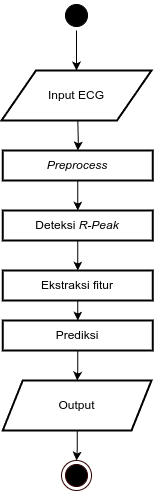
\includegraphics[width=.24\linewidth]{img/lstm-app flow.drawio.pdf}
	\caption{Diagram alir aplikasi inferensi}
	\label{fig:flowchart-inferensi}
\end{figure}

Gambar \ref{fig:flowchart-inferensi} menunjukkan alur kerja aplikasi inferensi yang dirancang.
% Setelah pengguna mengunggah data ECG, data tersebut akan melalui tahap \textit{preprocessing}, deteksi R-peak, ekstraksi fitur, prediksi, dan menghasilkan output hasil klasifikasi detak jantung.
Setelah pengguna mengunggah data ECG, aplikasi akan melakukan tahap \textit{preprocessing}, deteksi R-peak, ekstraksi fitur, klasifikasi, dan menghasilkan output hasil klasifikasi detak jantung.
Output tersebut akan ditampilkan pada antarmuka aplikasi inferensi yang dapat diakses oleh pengguna.
% Preprocessing dan deteksi R-peak penting dilakukan karena data rekaman ecg yang digunakan untuk inferensi belum terdapat anotasi pada titik R-peak.
Berbeda dengan tahap pelatihan, pada tahap inferensi, data ECG yang diunggah belum memiliki anotasi R-peak.
Oleh karena itu, perlu dilakukan tahap \textit{preprocessing} dan deteksi R-peak sebelum data dapat digunakan untuk klasifikasi detak jantung.

\begin{figure}[H]
	\centering
	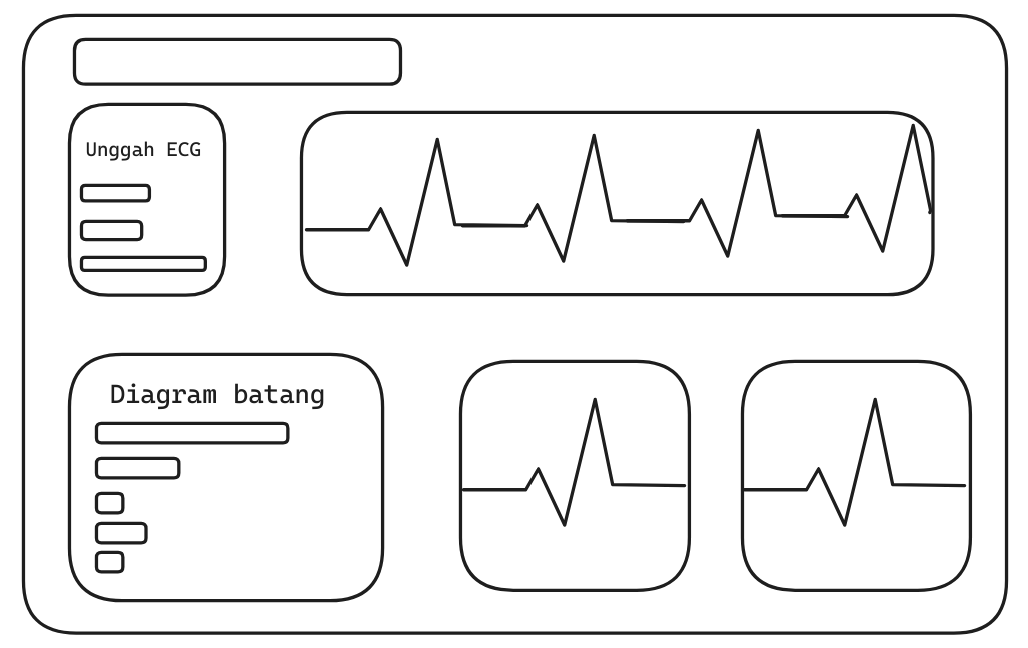
\includegraphics[width=.8\textwidth]{img/2024-06-24_12-19.png}
	\caption{Desain antarmuka aplikasi inferensi}
	\label{fig:lofi-inferensi}
\end{figure}

% --- perancangan antarmuka aplikasi
Gambar \ref{fig:lofi-inferensi} menunjukkan desain antarmuka aplikasi inferensi yang dirancang.
Antarmuka aplikasi terdiri dari dua bagian utama, yaitu bagian input dan bagian output.
Pada bagian input, pengguna dapat mengunggah data ECG yang akan digunakan untuk klasifikasi detak jantung.
Pengguna juga dapat memilih model yang akan digunakan untuk klasifikasi.
% Pada bagian output, dibagi menjadi tiga bagian, yaitu visualisasi data ECG, hasil klasifikasi berupa diagram batang, dan contoh sinyal ECG detak jantung pada setiap kelas.
Pada bagian output, terbagi menjadi tiga bagian.
Bagian pertama menampilkan visualisasi data ECG yang diunggah oleh pengguna.
Bagian kedua menampilkan hasil klasifikasi detak jantung dalam bentuk diagram batang.
Bagian terakhir menampilkan sampel sinyal ECG detak jantung pada setiap kelas yang telah diklasifikasikan oleh model.





% %%%%%%%%%%%%%%%%%%%%%%%%%%%%%%%%%%%%%%%%%%%%%%%%%%%%%%%%%%%%%%%%%%%%%%%
% BAB 5 IMPLEMENTASI DAN PENGUJIAN
%%%%%%%%%%%%%%%%%%%%%%%%%%%%%%%%%%%%%%%%%%%%%%%%%%%%%%%%%%%%%%%%%%%%%%%
%
%
% model h5 diubah dulu ke tflite
% untuk inferensi, dibuat aplikasi web menggunakan flask
% aplikasi web ini bisa diakses oleh user
% user mengupload file rekam ecg kemudian nanti hasilnya akan ditampilkan
% aplikasinya dideploy pada raspi5 dan intel nuc
% nanti akan diuji performanya dengan cara menghitung waktu inferensi dan memory usage
% pengujian inferensinya dilakukan dengan menggunakan dataset ecg dengan panjang 10 detik sejumlah 5 kali, panjang 1 menit sejumlah 5 kali, dan panjang 10 menit sejumlah 5 kali
% pengujian memory dilakukan dengan memantau memory usage maksimum yang digunakan oleh aplikasi ketika melakukan inferensi
% pengujian waktu inferensi dilakukan dengan memantau waktu yang dibutuhkan oleh aplikasi untuk melakukan inferensi mulai dari aplikasi menerima file rekam ecg hingga menghasilkan output
% dari masing-masing 5 kali pengujian, diambil rata-rata waktu inferensi dan memory usage
% 
%
%

\mychapter{5}{BAB 5 IMPLEMENTASI DAN PENGUJIAN}
Pada bab ini akan dijelaskan implementasi dari model yang telah dilatih sebelumnya serta pengujian performa inferensi model yang dilakukan pada perangkat tepi.
Terdapat tiga tahapan yang dilakukan, yaitu konversi model dari format H5 ke TFLite, implementasi aplikasi web untuk melakukan inferensi, dan pengujian performa inferensi pada perangkat tepi.
% Tahapan implementasi meliputi konversi model dari format H5 ke TFLite, pembuatan aplikasi web untuk melakukan inferensi, dan pengujian performa inferensi pada perangkat tepi.

\section{Konversi Model ke TFLite}
% from tensorflow.keras.models import load_model
% import tensorflow as tf
% for model_path in model_list:
%   model = load_model(model_path)
%   converter = tf.lite.TFLiteConverter.from_keras_model(model)
%   converter._experimental_default_to_single_batch_in_tensor_list_ops = True
%   converter.optimizations = [tf.lite.Optimize.DEFAULT]
%   tflite_model = converter.convert()
%   open(model_path.replace('.h5', '.tflite'), 'wb').write(tflite_model)

Model yang telah dilatih dengan menggunakan TensorFlow sebelumnya memiliki format H5.
Format H5 merupakan format yang belum dioptimasi sehingga memiliki ukuran yang besar dan tidak efisien untuk dijalankan pada perangkat yang memiliki keterbatasan sumber daya.
Untuk itu, model yang telah dilatih perlu
diubah ke format TensorFlow Lite (TFLite) agar dapat dijalankan pada perangkat yang memiliki keterbatasan sumber daya.
TFLite merupakan format yang dioptimasi untuk dijalankan pada perangkat yang memiliki keterbatasan sumber daya.
Selain itu, TFLite juga memiliki ukuran yang lebih kecil dan dependensi yang lebih sedikit dibandingkan dengan model TensorFlow biasa.

% dont include code in the main text, put it in the appendix
Untuk mengubah model dari format H5 ke TFLite, digunakan TFLiteConverter yang disediakan oleh TensorFlow.
TFLiteConverter adalah sebuah API yang disediakan oleh TensorFlow untuk mengubah model TensorFlow ke format TFLite.
Pada proses konversi, dilakukan optimisasi dengan cara kuantisasi.
Kuantisasi adalah teknik yang digunakan untuk mengurangi presisi dari angka yang digunakan untuk merepresentasikan parameter dari model.
Dengan mengurangi presisi, ukuran model dapat dikurangi dan dapat meningkatkan performa dan efisiensi inferensi model.
% Kuantisasi yang digunakan yaitu Dynamic range quantization. Dynamic range quantization is a recommended starting point because it provides reduced memory usage and faster computation without having to provide a representative dataset for calibration. 
Kuantisasi yang digunakan adalah \textit{Dynamic range quantization}.
\textit{Dynamic range quantization} mampu mengurangi penggunaan memori dan meningkatkan kecepatan komputasi tanpa perlu menyediakan dataset representatif untuk kalibrasi.

% Secara default, konversi model lstm ke format tflite memiliki dynamic batch size dan memerlukan ops default tensorflow, sehingga memerlukan dependensi tensorflow untuk menggunakannya. Agar dapat digunakan hanya dengan dependensi tflite runtime make perlu untuk mengubah batch size menjadi = 1.
Ketika model LSTM dikonversi ke format TFLite, model tersebut menggunakan
% dynamic batch size 
ukuran batch yang dinamis
% dan memerlukan \textit{ops} bawaan TensorFlow.
% gunakan bahasa indonesia sederhana, jangan istilah
dan memerlukan operasi bawaan TensorFlow.
Hal ini menyebabkan model TFLite tersebut memerlukan dependensi TensorFlow untuk dijalankan.
Untuk menghindari dependensi TensorFlow, batch size pada model TFLite perlu diubah menjadi 1.
Dengan mengubah batch size menjadi 1, model TFLite dapat dijalankan tanpa memerlukan dependensi TensorFlow.

% --- tabel komparasi ukuuran model sebelum dan sesudah konversi ---
% lstm-512 14.3M 1.2M
% lstm-256 3.6M 318.5k
% bi-lstm 8.0M 694.4k
% lstm-fcn 3.4M 299.4k

\begin{table}[H]
  \centering
  \caption{Perbandingan ukuran model sebelum dan sesudah konversi}
  \label{tab:ukuran-model}
  \begin{tabularx}{0.8\textwidth} {
    | >{\centering\arraybackslash}X
    | >{\centering\arraybackslash}X
    | >{\centering\arraybackslash}X | }
    \hline
    \textbf{Model} & \textbf{Ukuran (H5)} & \textbf{Ukuran (TFLite)} \\
    \hline
    LSTM-512 & 14,3 MB & 1,2 MB \\
    \hline
    LSTM-256 & 3,6 MB & 318,5 KB \\
    \hline
    Bi-LSTM & 8,0 MB & 694,4 KB \\
    \hline
    LSTM-FCN & 3,4 MB & 299,4 KB \\
    \hline
  \end{tabularx}
\end{table}

Tabel \ref{tab:ukuran-model} menunjukkan perbandingan ukuran file model sebelum dan sesudah konversi ke format TFLite.
Dari tabel tersebut, dapat dilihat bahwa ukuran model setelah dikonversi ke format TFLite lebih kecil dibandingkan dengan ukuran model sebelum dikonversi.
Ukuran model berkurang hingga 90\% setelah dikonversi ke format TFLite.
Ukuran model yang lebih kecil ini dapat mengurangi penyimpanan yang dibutuhkan untuk menyimpan model.
Selain itu, ukuran model yang lebih kecil juga dapat 
mengurangi waktu yang dibutuhkan untuk memuat model ke memori dan
mengurangi penggunaan memori ketika melakukan inferensi.



\section{Implementasi Aplikasi Web}
% user -> upload -> preprocess -> rpeak detection -> feature extraction -> predict -> result

Untuk melakukan inferensi model, dibuat sebuah aplikasi berbasis web yang dapat diakses oleh pengguna.
Aplikasi web ini dibuat menggunakan Flask.
% Alur kerja aplikasi web ditunjukkan pada Gambar \ref{fig:alur-kerja-aplikasi-web}.
\textit{Sequence diagram} dari aplikasi web ditunjukkan pada Gambar \ref{fig:alur-kerja-aplikasi-web}.
Pengguna dapat mengunggah file rekaman ECG pada aplikasi web.
Setelah pengguna mengunggah file rekaman ECG, aplikasi web akan melakukan inferensi menggunakan model TFLite yang telah dikonversi sebelumnya.
Hasil prediksi kemudian akan ditampilkan pada pengguna.

\begin{figure}[H]
  \centering
  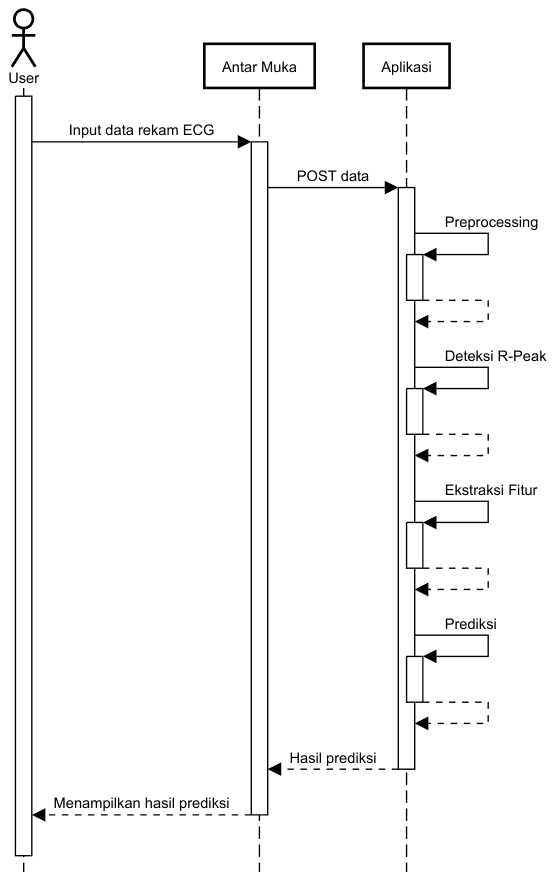
\includegraphics[width=0.6\textwidth]{img/sequence.png}
  \caption{\textit{Sequence diagram} aplikasi web}
  \label{fig:alur-kerja-aplikasi-web}
\end{figure}

% Gambar \ref{fig:aplikasi-web} menunjukkan tampilan aplikasi web yang dibuat.
Tampilan aplikasi web yang dibuat ditunjukkan pada Gambar \ref{fig:aplikasi-web}.
% Pengguna dapat mengunggah file rekaman ECG pada aplikasi web dan memilih model yang akan digunakan untuk melakukan prediksi.
% Tampilan aplikasi web terdiri dari beberapa bagian, yaitu bagian form input yang digunakan untuk mengunggah file rekaman ECG serta memilih model yang akan digunakan untuk melakukan prediksi, dan output yang akan menampilkan hasil prediksi yang terdiri dari diagram batang jumlah masing-masing kelas, tampilan sinyal ecg yang, dan tampilan sinyal pada masing-masing detak jantung.
Tampilan aplikasi web terdiri dari dua bagian utama, yaitu bagian input pengguna dan bagian output hasil prediksi.
Pada bagian input pengguna, pengguna dapat mengunggah file rekaman ECG dan memilih model yang akan digunakan untuk melakukan prediksi.
Pada bagian output hasil prediksi, terdapat tampilan output hasil prediksi yang terdiri dari diagram batang masing-masing kelas, tampilan keseluruhan sinyal ECG, dan tampilan sinyal ecg pada masing-masing detak jantung.
% Pengguna dapat mengunggah file rekaman ECG pada aplikasi web.
% Pengguna juga dapat memilih model yang akan digunakan untuk melakukan prediksi.
% Pengguna kemudian dapat menekan tombol \textit{Predict} untuk memulai proses prediksi.
Pada aplikasi web ini, pengguna dapat memilih model yang akan digunakan untuk melakukan prediksi.
Setelah pengguna mengunggah file rekaman ECG dan memilih model, pengguna dapat menekan tombol \textit{Predict} untuk memulai proses prediksi.
Setelah proses prediksi selesai, hasil prediksi akan ditampilkan pada pengguna.

% --- gambar ui aplikasi web ---
\begin{figure}[H]
  \centering
  % 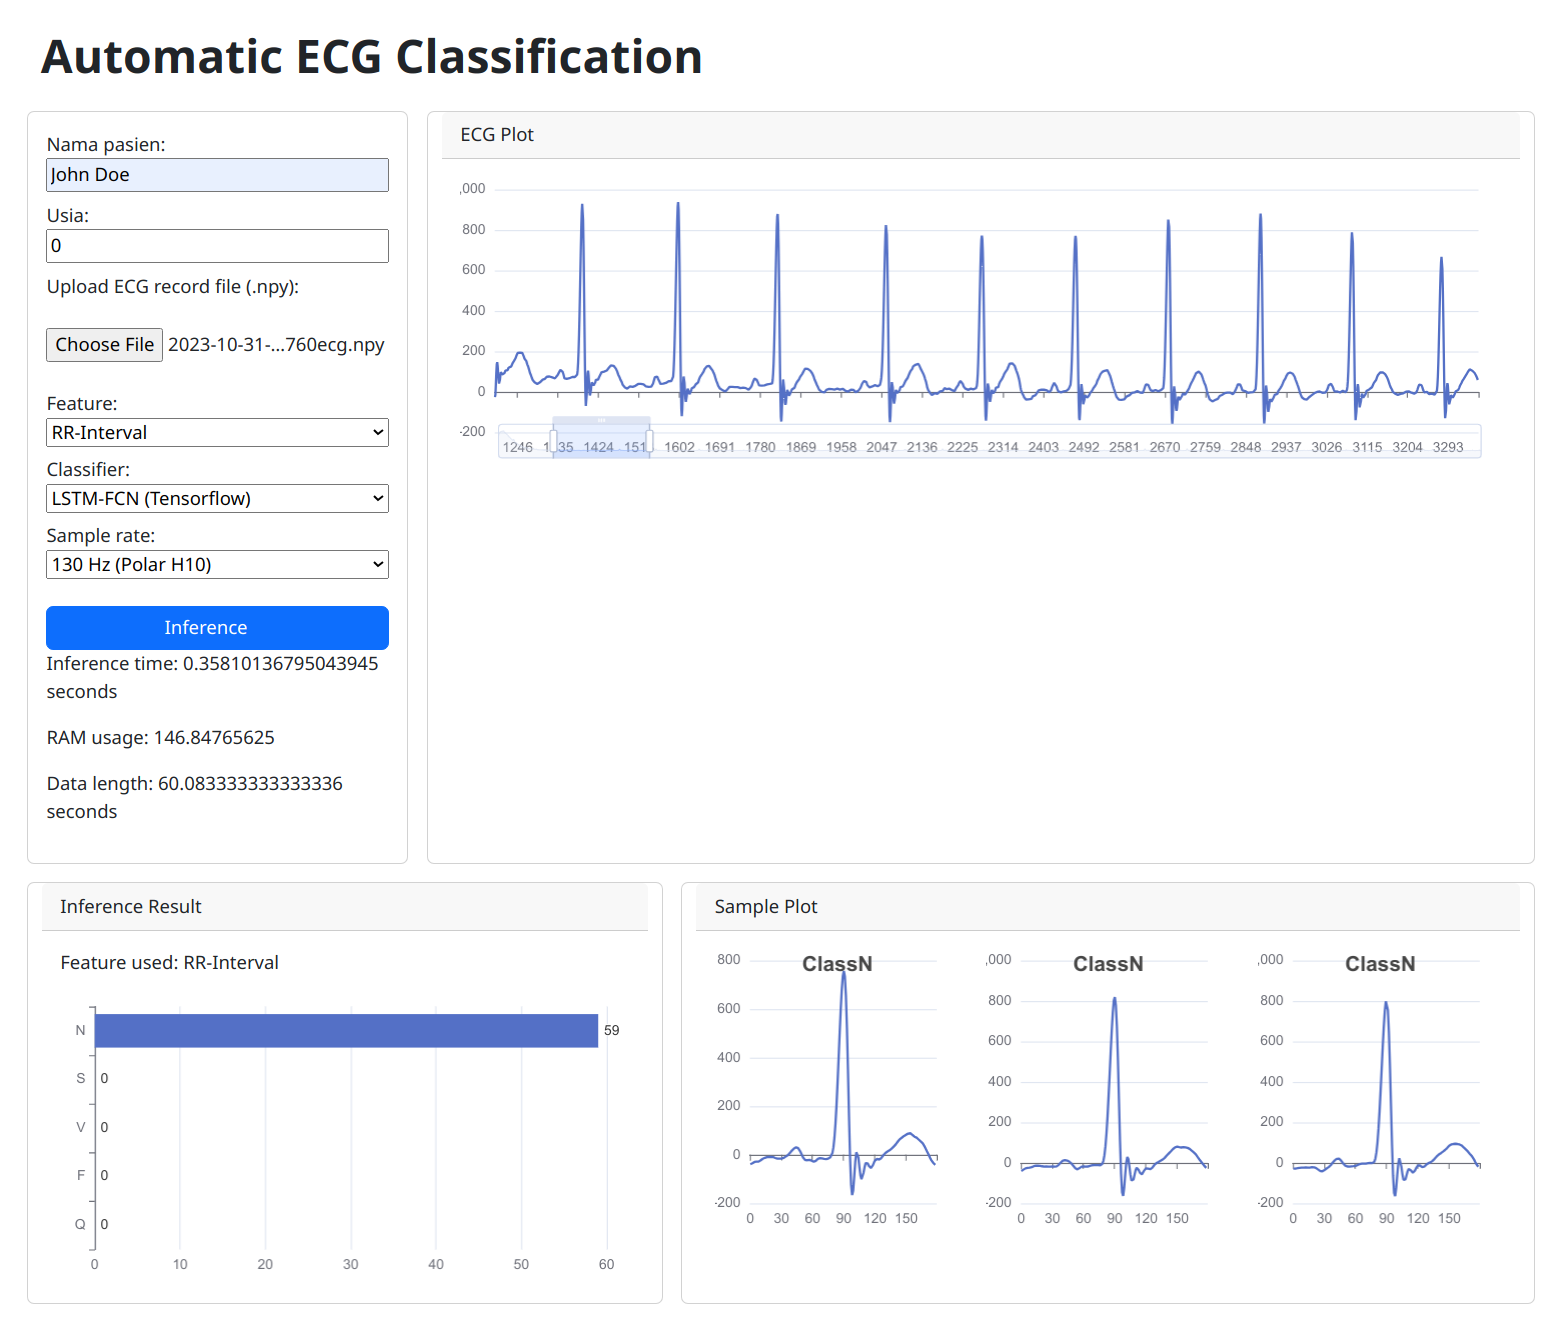
\includegraphics[width=0.8\textwidth]{img/tampilan-web.png}
  \fbox{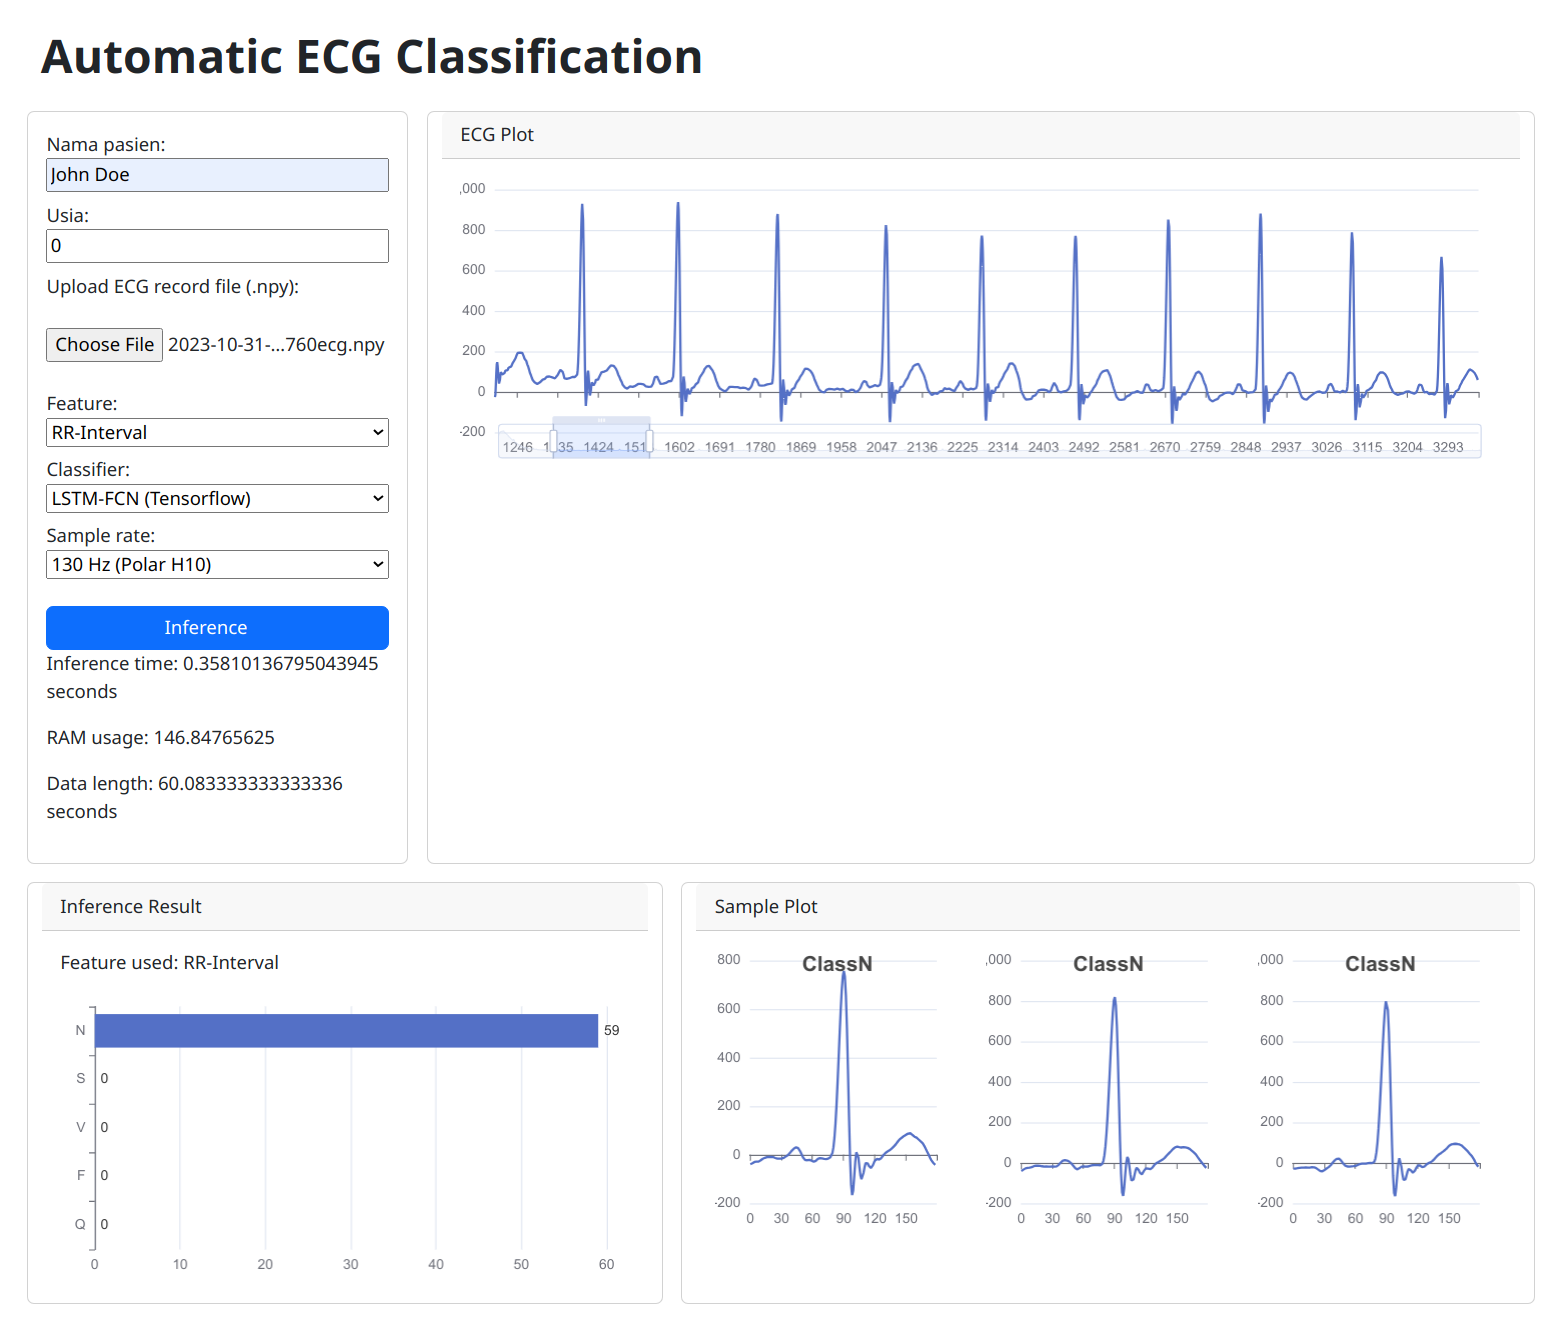
\includegraphics[width=0.9\textwidth]{img/tampilan-web.png}}
  \caption{Tampilan aplikasi web}
  \label{fig:aplikasi-web}
\end{figure}

% Proses inferensi terdiri dari beberapa tahap, yaitu \textit{preprocessing}, deteksi R-peak, ekstraksi fitur, dan prediksi.
Pada proses inferensi, terdapat beberapa tahapan yang dilakukan, yaitu \textit{preprocessing}, deteksi R-peak, ekstraksi fitur, dan prediksi.
% Sebelum data ECG dapat digunakan untuk melakukan prediksi, data ECG perlu diproses terlebih dahulu.
\textit{Preprocessing} dilakukan untuk membersihkan data dari gangguan dan mempersiapkan data untuk tahap selanjutnya.
Proses \textit{preprocessing} terdiri dari resampling, penghapusan \textit{noise} frekuensi tinggi menggunakan \textit{wavelet denoising}, penghapusan \textit{baseline wander}, dan normalisasi menggunakan \textit{z-score normalization}.
% --- pindahan dari bab 4 ---

% trained on 360hz mitboh but will be tested on 130hz polar h10
Data ECG yang akan digunakan untuk melakukan pengujian merupakan data yang direkam menggunakan perangkat Polar H10.
Data ECG yang direkam menggunakan perangkat Polar H10 tersebut memiliki frekuensi sampel 130 Hz, sedangkan dataset yang digunakan untuk melatih model memiliki frekuensi sampel 360 Hz.
% Sementara itu, model yang telah dilatih sebelumnya menggunakan dataset yang memiliki frekuensi sampel 360 Hz.
Oleh karena itu, data rekaman ECG perlu diubah ke dalam frekuensi sampel 360 Hz agar dapat digunakan untuk melakukan prediksi menggunakan model yang telah dilatih sebelumnya.
% using scipy resample
Data rekaman ECG diubah ke dalam frekuensi sampel 360 Hz menggunakan metode \textit{resampling}.
\textit{Resampling} dilakukan dengan menggunakan bantuan fungsi \textit{resample} yang disediakan oleh pustaka SciPy.
% dengan jumlah target sampel yang dihitung menggunakan persamaan \ref{eq:resample}
% \begin{equation}
%     N_{\text{target}} = \frac{360}{130} \times N_{\text{asal}}
%     \label{eq:resample}
% \end{equation}
% dengan $N_{\text{target}}$ dan $N_{\text{asal}}$ masing-masing menunjukkan jumlah sampel target dan jumlah sampel asal.


Selama proses pengambilan data, sinyal ECG rentan terhadap \textit{noise} berfrekuensi tinggi.
Frekuensi tinggi pada data ECG dianggap sebagai \textit{noise} yang dapat mengganggu proses klasifikasi detak jantung.
Pada penelitian ini, \textit{noise} berfrekuensi tinggi dihilangkan dengan menggunakan metode \textit{wavelet denoise}.
\textit{Wavelet denoise} menghilangkan \textit{noise} pada sinyal maupun gambar dengan menggunakan \textit{wavelet transform}.
\textit{Wavelet transform} memungkinkan sinyal untuk dipecah menjadi beberapa bagian frekuensi yang berbeda, sehingga memungkinkan penghilangan \textit{noise} pada frekuensi tertentu.
Metode \textit{wavelet denoise} yang digunakan pada penelitian ini adalah \textit{VisuShrink} dengan mode \textit{soft thresholding}, dan menggunakan \textit{wavelet} Daubechies 8 (db8) dengan 10 level \textit{wavelet decomposition}.

% --- dijelaskan lebih detail? ---

% Sinyal ECG diubah ke dalam domain \textit{wavelet} dengan menggunakan \textit{wavelet transform} Daubechies 8 (db8) dengan 10 level \textit{wavelet decomposition}.
% \textit{Noise} pada sinyal ECG kemudian dapat dihilangkan dengan mengurangi koefisien \textit{wavelet} yang memiliki nilai di bawah ambang batas tertentu.

%
% Setelah menghilangkan \textit{noise} berfrekuensi tinggi, tahap selanjutnya adalah menghilangkan \textit{baseline wander} (BW).
% elaborate
Selain \textit{noise} berfrekuensi tinggi, sinyal ECG juga rentan terhadap \textit{baseline wander}.
\textit{Baseline wander} (BW) merupakan \textit{noise} berfrekuensi rendah yang terdapat pada ECG.
BW dapat disebabkan oleh beberapa faktor, seperti pernapasan, elektroda yang bermuatan listrik, dan gerakan dari pasien \parencite{lenisComparisonBaselineWander2017}.
% metode baseline wander
        % baseline = medfilt(ecg, 71)
        % baseline = medfilt(baseline, 215)
        %
        % # Remove Baseline
        % for i in range(0, len(ecg)):
        %     ecg[i] = ecg[i] - baseline[i]
% BW dihilangkan dengan menggunakan metode \textit{median filter} dengan panjang jendela 71 dan 215.
BW dihilangkan dengan melakukan substraksi antara sinyal ECG dengan \textit{trend} sinyal.
\textit{Trend} sinyal diperoleh dengan menggunakan metode \textit{median filter} sebanyak dua kali dengan panjang jendela 71 dan 215.
% Median filtering, as mentioned earlier, is another method commonly used for baseline wander removal. It involves replacing each data point in the signal with the median value within a specified window around that point. This approach can effectively remove baseline variations while preserving the shape of the ECG waveform.
\textit{Median filter} akan menggantikan setiap titik data pada sinyal dengan nilai median dalam jendela yang ditentukan.
\textit{Median filter} didefinisikan oleh persamaan \ref{eq:median-filter}
\begin{equation}
    % perlu dicek lagi
    y[n] = \text{median}(x[n - \frac{M}{2} : n + \frac{M}{2}])
    \label{eq:median-filter}
\end{equation}
dengan $y[n]$ adalah sinyal hasil \textit{median filter}, $x[n]$ adalah sinyal asli, dan $M$ adalah panjang jendela \textit{median filter}.
% Yang mana $y[n]$, $x[n]$, dan $M$ masing-masing menunjukkan sinyal hasil \textit{median filter}, sinyal asli, dan panjang jendela \textit{median filter}.

% Setelah \textit{baseline wander} dihilangkan, data dinormalisasi untuk menghindari perbedaan skala.
% Setelah \textit{nose} dan \textit{baseline wander} dihilangkan, data dinormalisasi untuk menghindari perbedaan skala.
% Normalisasi yang dilakukan yaitu \textit{Z-score normalization}.
% metode normalisasi
Setelah \textit{noise} dan \textit{baseline wander} dihilangkan, tahap selanjutnya adalah normalisasi data.
Normalisasi dilakukan untuk menghindari adanya perbedaan skala pada data.
Metode normalisasi yang digunakan pada penelitian ini adalah \textit{Z-score normalization}.
\textit{Z-score normalization} mengubah data ke dalam distribusi normal dengan rata-rata 0 dan standar deviasi 1.
\textit{Z-score normalization} didefinisikan oleh persamaan \ref{eq:z-score}
\begin{equation}
		z = \frac{x - \mu}{\sigma}
		\label{eq:z-score}
\end{equation}
dengan $z$ adalah data yang telah dinormalisasi, $x$ adalah data asli, $\mu$ adalah rata-rata data, dan $\sigma$ adalah standar deviasi data.


\begin{figure}[H]
    \centering
    \fbox{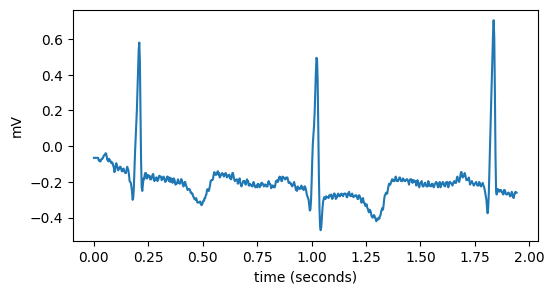
\includegraphics[width=0.7\linewidth]{./img/sebelum_prep.png}}
    % 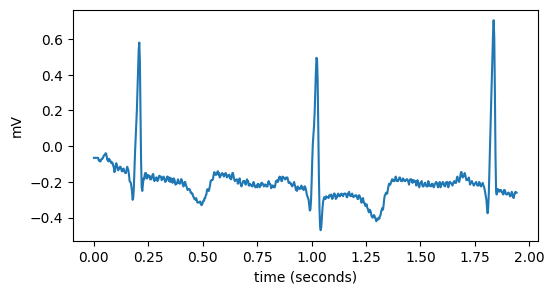
\includegraphics[width=0.6\linewidth]{./img/sebelum_prep.png}
	\caption{Data sebelum \textit{preprocessing}}
	\label{fig:sebelum-prep}
\end{figure}

\begin{figure}[H]
  \centering
  \fbox{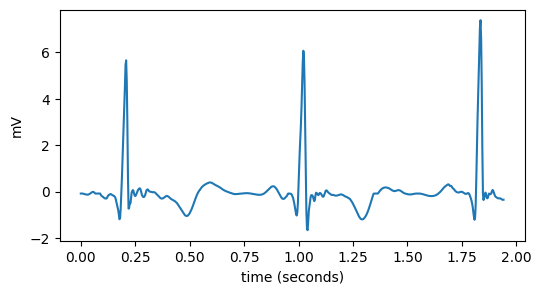
\includegraphics[width=0.7\linewidth]{./img/setelah_prep.png}}
  % 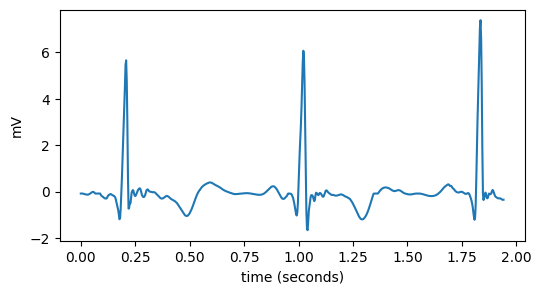
\includegraphics[width=0.6\linewidth]{./img/setelah_prep.png}
  \caption{Data setelah \textit{preprocessing}}
  \label{fig:setelah-prep}
\end{figure}


% Gambar \ref{fig:sebelum-prep} menunjukkan data sebelum dilakukan \textit{preprocessing}, sedangkan Gambar \ref{fig:setelah-prep} menunjukkan data setelah dilakukan \textit{preprocressing}.
Gambar \ref{fig:sebelum-prep} dan \ref{fig:setelah-prep} memperlihatkan perbandingan data ECG sebelum dan setelah dilakukan \textit{preprocessing}.
% Pada Gambar \ref{fig:sebelum-prep}, terlihat bahwa terdapat \textit{noise} berfrekuensi tinggi dan variasi pada \textit{baseline} sinyal ECG.
Pada Gambar \ref{fig:sebelum-prep}, terlihat bahwa pada data ECG masih terdapat gangguan seperti \textit{noise} berfrekuensi tinggi dan variasi pada \textit{baseline} sinyal.
% Setelah dilakukan \textit{preprocessing}, sinyal ECG menjadi lebih halus dan memiliki baseline yang lebih rata.
Setelah dilakukan \textit{preprocessing}, sinyal ECG menjadi lebih halus dan memiliki \textit{baseline} yang lebih rata, seperti yang terlihat pada Gambar \ref{fig:setelah-prep}.

% ---

% Setelah proses \textit{preprocessing} selesai, dilakukan deteksi R-peak menggunakan algoritma Pan-Tompkins untuk menentukan posisi R-peak pada sinyal ECG.
Setelah proses \textit{preprocessing} selesai, dilakukan deteksi R-peak untuk menentukan posisi R-peak pada sinyal ECG.
Deteksi R-peak dilakukan dengan menggunakan algoritma Pan-Tompkins.
Algoritma Pan-Tompkins adalah algoritma yang digunakan untuk mendeteksi R-peak pada sinyal ECG \parencite{panRealtimeQRSDetection1985}.
% Keluaran dari deteksi R-peak adalah posisi R-peak pada sinyal ECG.
Dari posisi R-peak yang dideteksi, dihitung jarak antar R-peak untuk mendapatkan RR-interval.
RR-Interval ini kemudian diekstraksi menjadi 9 fitur seperti yang telah dijelaskan pada Subbab \ref{subsec: bab4-ekstraksi-fitur}.
Fitur-fitur ini kemudian digunakan sebagai input untuk model yang telah dilatih sebelumnya.
Aplikasi web akan melakukan prediksi menggunakan model yang telah dilatih sebelumnya dan menampilkan hasil prediksi pada pengguna.


\section{Pengujian Performa Inferensi}
% pengujian dilakukan dengan cara menghitung waktu inferensi dan memory usage
% pengujian dilakukan dengan menggunakan dataset ecg dengan panjang 10 detik sejumlah 5 kali, panjang 1 menit sejumlah 5 kali, dan panjang 10 menit sejumlah 5 kali
% dari masing-masing 5 kali pengujian, diambil rata-rata waktu inferensi dan memory usage
% pengujian dilakukan pada raspi4 dan intel nuc
% hasil pengujian waktu inferensi dan memory usage akan dibandingkan antara raspi5 dan intel nuc
Pengujian performa inferensi dilakukan untuk mengevaluasi efisiensi dan performa model dalam melakukan inferensi.
Pengujian performa inferensi dilakukan dengan menghitung waktu inferensi dan penggunaan memori yang digunakan oleh aplikasi saat melakukan inferensi.
Waktu inferensi dihitung dari saat aplikasi menerima file rekaman ECG hingga menghasilkan output prediksi.
Penggunaan memori dihitung dari memori maksimum yang digunakan oleh aplikasi saat melakukan inferensi.

Pengujian dilakukan pada dua perangkat tepi, yaitu Raspberry Pi 4 Model B dan Intel NUC.
% Raspberry Pi 4 Model B dilengkapi dengan prosesor ARM Cortex-A72 4-core 1.8 GHz dan RAM 8 GB LPDDR4.
Raspberry Pi 4 Model B yang digunakan pada penelitian ini dilengkapi dengan prosesor ARM Cortex-A72 4-core 1.8 GHz dan RAM 8 GB LPDDR4.
% Sementara itu, Intel NUC menggunakan prosesor Intel Core i3-1115G4 2-core 4-thread 4.1 GHz dan RAM 16 GB DDR4.
Sementara itu, Intel NUC yang digunakan pada penelitian ini dilengkapi dengan prosesor Intel Core i3-1115G4 2-core 4-thread 4.1 GHz dan RAM 16 GB DDR4.
Pada perangkat Raspberry Pi 4 Model B, sistem operasi yang digunakan adalah Raspberry Pi OS Lite, sedangkan pada Intel NUC, sistem operasi yang digunakan adalah Debian yang berjalan pada Windows Subsystem for Linux (WSL).
% Kedua perangkat ini memiliki spesifikasi yang berbeda terutama pada arsitektur prosesor.
% Raspberry Pi 4 Model B menggunakan arsitektur ARM sementara Intel NUC menggunakan arsitektur x86.
% Pengujian pada dua perangkat ini dapat memberikan gambaran kinerja aplikasi pada perangkat dengan arsitektur dan spesifikasi yang berbeda.

Pengujian dilakukan dengan tiga skenario, yaitu pengujian dengan data ECG berdurasi 10 detik, 1 menit, dan 10 menit. 
Pada masing-masing skenario, dilakukan pengujian sebanyak lima kali dengan menggunakan data ECG yang berbeda.
Dari masing-masing lima kali pengujian, diambil rata-rata waktu inferensi dan rata-rata penggunaan memori maksimum.
Hasil pengujian ini akan digunakan untuk mengevaluasi efisiensi dan performa aplikasi dalam melakukan inferensi pada kedua perangkat.
% Masing-masing skenario diulang sebanyak lima kali untuk mendapatkan hasil yang konsisten.
% Dari setiap lima kali pengujian, diambil rata-rata waktu inferensi dan rata-rata penggunaan memori maksimum. 
% Hasil pengujian ini akan digunakan untuk mengevaluasi efisiensi dan performa aplikasi dalam melakukan inferensi pada kedua perangkat.
%

% %%%%%%%%%%%%%%%%%%%%%%%%%%%%%%%%%%%%%%%%%%%%%%%%%%%%%%%%%%%%%%%%%%%%%%%
% BAB 6
%%%%%%%%%%%%%%%%%%%%%%%%%%%%%%%%%%%%%%%%%%%%%%%%%%%%%%%%%%%%%%%%%%%%%%%





\mychapter{6}{BAB 6 HASIL DAN PEMBAHASAN}



% --- hasil evaluasi akurasi, presisi, recall, dan f1 score ---
Hasil evaluasi akurasi, presisi, recall, dan f1 score dari model LSTM-512, LSTM-256, BiLSTM, dan LSTM-FCN ditunjukkan pada Tabel \ref{tab:evaluasi}.
% Dari hasil evaluasi, seluruh model mampu melakukan klasifikasi dengan akurasi di atas 0.96.
Dari hasil evaluasi, model LSTM-512 memiliki akurasi, presisi, recall, dan f1 score tertinggi dibandingkan dengan model LSTM-256, BiLSTM, dan LSTM-FCN.
Model LSTM-512 memiliki akurasi sebesar 0,9679, presisi sebesar 0,9662, recall sebesar 0,9679, dan f1 score sebesar 0,9652.
Meskipun demikian, model LSTM-256, BiLSTM, dan LSTM-FCN juga mendapatkan hasil evaluasi yang baik dengan akurasi, presisi, recall, dan f1 score di atas 0,96.
Akurasi, presisi, recall, dan f1 score pada seluruh model memiliki selisih yang tidak signifikan dengan selisih maksimal sebesar 0,0046.

\begin{table}[H]
  \centering
  \caption{Hasil evaluasi akurasi, presisi, recall, dan f1 score}
  \label{tab:evaluasi}
  % \begin{tabular}{|c|c|c|c|c|}
  \begin{tabularx}{0.8\textwidth}{
      |>{\centering\arraybackslash}X
      |>{\centering\arraybackslash}X
      |>{\centering\arraybackslash}X
      |>{\centering\arraybackslash}X
      |>{\centering\arraybackslash}X|}
    \hline
    \textbf{Model} & \textbf{Akurasi} & \textbf{Presisi} & \textbf{Recall} & \textbf{F1 Score} \\ \hline
    LSTM-512       & \textbf{0,9679}           & \textbf{0,9662}          & \textbf{0,9679}         & \textbf{0,9652}           \\ 
    \hline
    LSTM-256       & 0,9674           & 0,9656          & 0,9674         & 0,9645           \\ 
    \hline
    BiLSTM         & 0,9636           & 0,9617          & 0,9636         & 0,9606           \\ 
    \hline
    LSTM-FCN       & 0,9667           & 0,9643          & 0,9667         & 0,9643           \\ \hline
  \end{tabularx}
\end{table}

% --- confussion matrix ---
Hasil evaluasi berupa \textit{confusion matrix} dari model LSTM-512, LSTM-256, BiLSTM, dan LSTM-FCN ditunjukkan pada Tabel \ref{tab:confusion-lstm512}, Tabel \ref{tab:confusion-lstm256}, Tabel \ref{tab:confusion-bilstm}, dan Tabel \ref{tab:confusion-lstmfcn}.
Dari hasil \textit{confusion matrix}, dapat dilihat bahwa model LSTM-512, LSTM-256, BiLSTM, dan LSTM-FCN memiliki kemampuan yang baik dalam melakukan klasifikasi detak jantung normal (N).
Akan tetapi, model LSTM-512, LSTM-256, BiLSTM, dan LSTM-FCN memiliki kesulitan dalam melakukan klasifikasi detak jantung jenis lain terutama detak jantung \textit{fusion} (F) dan detak jantung \textit{unknown} (Q).
Hal ini dapat dilihat dari rasio misklasifikasi pada detak jantung \textit{fusion} (F) dan detak jantung \textit{unknown} (Q) yang cukup tinggi dibandingkan dengan detak jantung lainnya.
% model cendurung mengklasifikasikan ke kelas n yang menunjukkan overfitting ke kelas n
Ketika model melakukan kesalahan klasifikasi, model cenderung mengklasifikasikan detak jantung ke kelas normal (N) yang menunjukkan adanya overfitting ke kelas normal (N).
Hal ini dapat disebabkan karena adanya ketidakseimbangan jumlah detak jantung pada masing-masing kelas pada dataset yang digunakan.
% yang menyebabkan model cenderung mengklasifikasikan detak jantung ke kelas yang mayoritas.
Ketidakseimbangan tersebut menyebabkan model cenderung mengklasifikasikan detak jantung ke kelas yang mayoritas.


\begin{table}[H]
  \centering
  \caption{Confusion matrix model LSTM-512}
  \label{tab:confusion-lstm512}
  % \begin{tabular}{cc|ccccc}
  %   \multicolumn{2}{c}{} & \multicolumn{5}{c}{Prediksi} \\
  %   & & N & S & V & F & Q \\ \hline
  %   \multirow{5}{*}{\rotatebox[origin=c]{90}{Aktual}}
  %   & N & 25722 & 25 & 166 & 7 & 0 \\
  %   & S & 88 & 641 & 79 & 0 & 0 \\
  %   & V & 335 & 36 & 1581 & 2 & 0 \\
  %   & F & 183 & 0 & 6 & 47 & 0 \\
  %   & Q & 1 & 1 & 0 & 0 & 0 \\ \hline
  % \end{tabular}
  \begin{tabularx}{0.6\textwidth}{|c
      |>{\centering\arraybackslash}X
      |>{\centering\arraybackslash}X
      |>{\centering\arraybackslash}X
      |>{\centering\arraybackslash}X
      |>{\centering\arraybackslash}X|}
    \hline
    \multirow{2}{*}{\textbf{Aktual}} & \multicolumn{5}{c|}{\textbf{Prediksi}} \\
    \cline{2-6}
               & \textbf{N} & \textbf{S} & \textbf{V} & \textbf{F} & \textbf{Q} \\ \hline
               \textbf{N} & 25722 & 25 & 166 & 7 & 0 \\
    \hline
              \textbf{S} & 88 & 641 & 79 & 0 & 0 \\
    \hline
              \textbf{V} & 335 & 36 & 1581 & 2 & 0 \\
    \hline
              \textbf{F} & 183 & 0 & 6 & 47 & 0 \\
    \hline
              \textbf{Q} & 1 & 1 & 0 & 0 & 0 \\ \hline
  \end{tabularx}
\end{table}

\begin{table}[H]
  \centering
  \caption{Confusion matrix model LSTM-256}
  \label{tab:confusion-lstm256}
  % \begin{tabular}{cc|ccccc}
  %   \multicolumn{2}{c}{} & \multicolumn{5}{c}{Prediksi} \\
  %   & & N & S & V & F & Q \\ \hline
  %   \multirow{5}{*}{\rotatebox[origin=c]{90}{Aktual}}
  %   & N & 25748 & 24 & 140 & 8 & 0 \\
  %   & S & 83 & 644 & 81 & 0 & 0 \\
  %   & V & 360 & 56 & 1538 & 0 & 0 \\
  %   & F & 182 & 0 & 8 & 46 & 0 \\
  %   & Q & 1 & 0 & 1 & 0 & 0 \\ \hline
  % \end{tabular}
  \begin{tabularx}{0.6\textwidth}{|c
      |>{\centering\arraybackslash}X
      |>{\centering\arraybackslash}X
      |>{\centering\arraybackslash}X
      |>{\centering\arraybackslash}X
      |>{\centering\arraybackslash}X|}
    \hline
    \multirow{2}{*}{\textbf{Aktual}} & \multicolumn{5}{c|}{\textbf{Prediksi}} \\
    \cline{2-6}
               & \textbf{N} & \textbf{S} & \textbf{V} & \textbf{F} & \textbf{Q} \\ \hline
               \textbf{N} & 25748 & 24 & 140 & 8 & 0 \\
    \hline
              \textbf{S} & 83 & 644 & 81 & 0 & 0 \\
    \hline
              \textbf{V} & 360 & 56 & 1538 & 0 & 0 \\
    \hline
              \textbf{F} & 182 & 0 & 8 & 46 & 0 \\
    \hline
              \textbf{Q} & 1 & 0 & 1 & 0 & 0 \\ \hline
  \end{tabularx}
\end{table}

\begin{table}[H]
  \centering
  \caption{Confusion matrix model BiLSTM}
  \label{tab:confusion-bilstm}
  % \begin{tabular}{cc|ccccc}
  %   \multicolumn{2}{c}{} & \multicolumn{5}{c}{Prediksi} \\
  %   & & N & S & V & F & Q \\ \hline
  %   \multirow{5}{*}{\rotatebox[origin=c]{90}{Aktual}}
  %   & N & 25684 & 40 & 190 & 6 & 0 \\
  %   & S & 94 & 627 & 87 & 0 & 0 \\
  %   & V & 397 & 45 & 1511 & 1 & 0 \\
  %   & F & 183 & 0 & 9 & 44 & 0 \\
  %   & Q & 1 & 0 & 1 & 0 & 0 \\ \hline
  % \end{tabular}
  \begin{tabularx}{0.6\textwidth}{|c
      |>{\centering\arraybackslash}X
      |>{\centering\arraybackslash}X
      |>{\centering\arraybackslash}X
      |>{\centering\arraybackslash}X
      |>{\centering\arraybackslash}X|}
    \hline
    \multirow{2}{*}{\textbf{Aktual}} & \multicolumn{5}{c|}{\textbf{Prediksi}} \\
    \cline{2-6}
               & \textbf{N} & \textbf{S} & \textbf{V} & \textbf{F} & \textbf{Q} \\ \hline
               \textbf{N} & 25684 & 40 & 190 & 6 & 0 \\
    \hline
               \textbf{S} & 94 & 627 & 87 & 0 & 0 \\
    \hline
               \textbf{V} & 397 & 45 & 1511 & 1 & 0 \\
    \hline
               \textbf{F} & 183 & 0 & 9 & 44 & 0 \\
    \hline
               \textbf{Q} & 1 & 0 & 1 & 0 & 0 \\ \hline
  \end{tabularx}
\end{table}

\begin{table}[H]
  \centering
  \caption{Confusion matrix model LSTM-FCN}
  \label{tab:confusion-lstmfcn}
  \begin{tabularx}{0.6\textwidth}{|c
      |>{\centering\arraybackslash}X
      |>{\centering\arraybackslash}X
      |>{\centering\arraybackslash}X
      |>{\centering\arraybackslash}X
      |>{\centering\arraybackslash}X|}
    \hline
    \multirow{2}{*}{\textbf{Aktual}} & \multicolumn{5}{c|}{\textbf{Prediksi}} \\
    \cline{2-6}
               & \textbf{N} & \textbf{S} & \textbf{V} & \textbf{F} & \textbf{Q} \\ \hline
               \textbf{N} & 25702 & 26 & 171 & 21 & 0 \\
    \hline
               \textbf{S} & 98 & 631 & 79 & 0 & 0 \\
    \hline
               \textbf{V} & 338 & 43 & 1571 & 2 & 0 \\
    \hline
               \textbf{F} & 175 & 0 & 8 & 53 & 0 \\
    \hline
               \textbf{Q} & 1 & 0 & 1 & 0 & 0 \\ \hline
  \end{tabularx}
\end{table}

% --- analisis hasil evaluasi akurasi, presisi, recall, dan f1 score ---


% --- hasil evaluasi waktu inferensi dan memory usage ---
\begin{table}[H]
\centering
\caption{Hasil evaluasi waktu inferensi dan penggunaan memori pada Raspberry Pi 4}
\label{tab:raspi4}
\begin{tabular}{|c|c|c|c|}
\hline
\textbf{Model} & \textbf{Durasi ECG} & \textbf{Waktu Inferensi (s)} & \textbf{Penggunaan Memori (MB)} \\ \hline
\multirow{3}{*}{ LSTM-512 }       & 10s                 & 0,1541                      & 131,1078                   \\ 
              \cline{2-4}
               & 1m                  & 1,0411                      & 135,0430                   \\
              \cline{2-4}
               & 10m                 & 14,0108                     & 180,4742                   \\ \hline
\multirow{3}{*}{ LSTM-256 }       & 10s                 & 0,1574                      & 131,0969                   \\ 
              \cline{2-4}
               & 1m                  & 0,9454                      & \textbf{134,2883}                   \\ 
              \cline{2-4}
               & 10m                 & 11,2050                     & 180,7773                   \\ \hline
\multirow{3}{*}{ BiLSTM }         & 10s                 & \textbf{0,1467}                      & 131,1070                   \\ 
              \cline{2-4}
               & 1m                  & 0,9615                      & 134,3352                   \\ 
              \cline{2-4}
               & 10m                 & 12,3639                     & \textbf{180,1117}                   \\ \hline
\multirow{3}{*}{ LSTM-FCN }       & 10s                 & 0,1916                      & \textbf{131,0898}                   \\
              \cline{2-4}
               & 1m                  & \textbf{0,8209}                      & 134,6477                   \\ 
              \cline{2-4}
               & 10m                 & \textbf{10,1330}                     & 180,3414                   \\ \hline
\end{tabular}
\end{table}

Tabel \ref{tab:raspi4} menunjukkan hasil evaluasi waktu inferensi dan penggunaan memori pada Raspberry Pi 4.
Pada skenario inferensi menggunakan data dengan durasi 10 detik, model BiLSTM memiliki waktu inferensi tercepat senilai 0,1467 detik.
Sementara itu, pada skenario inferensi menggunakan data dengan durasi 1 menit dan 10 menit, model LSTM-FCN memiliki waktu inferensi tercepat masing-masing senilai 0,8209 detik dan 10,1330 detik.
Tidak terdapat perbedaan yang signifikan pada penggunaan memori antara model LSTM-512, LSTM-256, BiLSTM, dan LSTM-FCN pada Raspberry Pi 4.
Penggunaan memori pada Raspberry Pi 4 pada inferensi menggunakan data dengan durasi 10 detik, 1 menit, dan 10 menit masing-masing sekitar 131 MB, 134 MB, dan 180 MB, dengan selisih kurang dari 1 MB.
Penggunaan memori tersebut masih dalam batas yang dapat diterima oleh Raspberry Pi 4 yang memiliki memori sebesar 8 GB.


\begin{table}[H]
\centering
\caption{Hasil evaluasi waktu inferensi dan penggunaan memori pada Intel NUC}
\label{tab:intelnuc}
\begin{tabular}{|c|c|c|c|}
\hline
\textbf{Model} & \textbf{Durasi ECG} & \textbf{Waktu Inferensi (s)} & \textbf{Penggunaan Memori (MB)} \\ \hline
\multirow{3}{*}{ LSTM-512 }       & 10s                 & 0,0360                      & 133,1211                   \\ 
              \cline{2-4}
               & 1m                  & 0,2760                      & 136,9086                   \\ 
              \cline{2-4}
               & 10m                 & 3,1574                      & \textbf{182,0367}                   \\ \hline
\multirow{3}{*}{ LSTM-256 }       & 10s                 & \textbf{0,0359}                      & \textbf{132,8539}                   \\
              \cline{2-4}
               & 1m                  & \textbf{0,2091}                      & \textbf{136,5195}                   \\ 
              \cline{2-4}
               & 10m                 & 2,2683                      & 182,2008                   \\ \hline
\multirow{3}{*}{ BiLSTM }         & 10s                 & 0,0371                      & 133,7625                   \\
              \cline{2-4}
               & 1m                  & 0,2360                      & 136,9438                   \\ 
              \cline{2-4}
               & 10m                 & 2,6397                      & 182,1641                   \\ \hline
\multirow{3}{*}{ LSTM-FCN }       & 10s                 & 0,0367                      & 133,6398                   \\
              \cline{2-4}
               & 1m                  & 0,2190                      & 137,0242                   \\
              \cline{2-4}
               & 10m                 & \textbf{1,9899}                      & 182,6266                   \\ \hline
\end{tabular}
\end{table}

Tabel \ref{tab:intelnuc} menunjukkan hasil evaluasi waktu inferensi dan penggunaan memori pada Intel NUC.
Pada skenario inferensi menggunakan data dengan durasi 10 detik dan 1 menit, model LSTM-256 memiliki waktu inferensi tercepat masing-masing senilai 0,0359 detik dan 0,2091 detik.
Sementara itu, pada skenario inferensi menggunakan data dengan durasi 10 menit, model LSTM-FCN memiliki waktu inferensi tercepat senilai 1,9899 detik.
Tidak terdapat perbedaan yang signifikan pada penggunaan memori antara model LSTM-512, LSTM-256, BiLSTM, dan LSTM-FCN pada Intel NUC.
Penggunaan memori pada Intel NUC pada inferensi menggunakan data dengan durasi 10 detik, 1 menit, dan 10 menit masing-masing sekitar 133 MB, 136 MB, dan 182 MB, dengan selisih kurang dari 1 MB.
Penggunaan memori tersebut masih dalam batas yang dapat diterima oleh Intel NUC yang memiliki memori sebesar 16 GB.

Berdasarkan hasil evaluasi waktu inferensi dan penggunaan memori pada Raspberry Pi 4 dan Intel NUC yang ditunjukkan pada Tabel \ref{tab:raspi4} dan Tabel \ref{tab:intelnuc}, dapat dilihat bahwa kecepatan waktu inferensi pada Intel NUC lebih cepat dibandingkan dengan Raspberry Pi 4.
Hal ini disebabkan oleh spesifikasi perangkat keras yang lebih tinggi pada Intel NUC dibandingkan dengan Raspberry Pi 4 terutama pada \textit{processor}.
% Terdapat perbedaan model yang memiliki waktu inferensi tercepat pada masing-masing perangkat.
% Pada Raspberry Pi 4, model BiLSTM memiliki waktu inferensi tercepat pada skenario inferensi menggunakan data dengan durasi 10 detik.
% Sementara itu, model LSTM-FCN memiliki waktu inferensi tercepat pada skenario inferensi menggunakan data dengan durasi 1 menit dan 10 menit.
% Pada Intel NUC, model LSTM-256 memiliki waktu inferensi tercepat pada skenario inferensi menggunakan data dengan durasi 10 detik dan 1 menit.
% Sementara itu, model LSTM-FCN memiliki waktu inferensi tercepat pada skenario inferensi menggunakan data dengan durasi 10 menit.
Sementara itu, penggunaan memori pada Raspberry Pi 4 dan Intel NUC memiliki selisih yang tidak signifikan.
Penggunaan memori pada Intel NUC sedikit lebih tinggi dibandingkan dengan Raspberry Pi 4 pada masing-masing skenario pengujian, dengan selisih sekitar 2 MB.




% --- tabel hasil prediksi pada pengujian ---
% model, pengujian ke-n, hasil prediksi (N, S, V, F, Q)
% ----------
% | Model | Pengujian ke | Hasil Prediksi |
% |       |        | N | S | V | F | Q |
% |-------|--------|----------------|
% 1 m								10m					
% lstm512	n	s	v	f	q			lstm512	n	s	v	f	q
% 1	59	0	0	0	0			1	978	0	0	0	0
% 2	62	0	0	0	0			2	969	0	0	0	0
% 3	62	0	0	0	0			3	969	0	0	0	0
% 4	60	0	0	0	0			4	969	0	0	0	0
% 5	58	0	0	0	0			5	969	0	0	0	0
% lstm256	n	s	v	f	q			lstm256	n	s	v	f	q
% 1	59	0	0	0	0			1	978	0	0	0	0
% 2	62	0	0	0	0			2	969	0	0	0	0
% 3	62	0	0	0	0			3	969	0	0	0	0
% 4	60	0	0	0	0			4	969	0	0	0	0
% 5	58	0	0	0	0			5	969	0	0	0	0
% bilstm	n	s	v	f	q			bilstm	n	s	v	f	q
% 1	59	0	0	0	0			1	978	0	0	0	0
% 2	62	0	0	0	0			2	969	0	0	0	0
% 3	62	0	0	0	0			3	969	0	0	0	0
% 4	60	0	0	0	0			4	969	0	0	0	0
% 5	58	0	0	0	0			5	969	0	0	0	0
% lstmfcn	n	s	v	f	q			lstmfcn	n	s	v	f	q
% 1	59	0	0	0	0			1	978	0	0	0	0
% 2	62	0	0	0	0			2	969	0	0	0	0
% 3	62	0	0	0	0			3	969	0	0	0	0
% 4	60	0	0	0	0			4	969	0	0	0	0
% 5	58	0	0	0	0			5	969	0	0	0	0

% -- tabel jumlah detak jantung yang diprediksi pada pengujian --
% durasi ecg, jumlah detak jantung yang diprediksi
% ----------

\begin{table}[H]
\centering
\caption{Jumlah detak jantung yang diprediksi pada pengujian}
\label{tab:jumlah-detak-jantung}
\begin{tabularx}{0.8\textwidth}{
  |>{\centering\arraybackslash}X
  |c
|}
\hline
\textbf{Durasi ECG} & \textbf{Jumlah Detak Jantung yang Diprediksi} \\ \hline
10s                 & 0                                              \\
\hline
1m                  & 301                                            \\
\hline
10m                 & 4854                                           \\ \hline
\end{tabularx}
\end{table}


% Tabel \ref{tab:jumlah-detak-jantung} menunjukkan jumlah detak jantung yang diprediksi selama pengujian pada data ECG dengan durasi 10 detik, 1 menit, dan 10 menit.
Tabel \ref{tab:jumlah-detak-jantung} menunjukkan jumlah total detak jantung yang diprediksi selama lima kali pengujian pada masing-masing skenario pengujian.
% Jumlah detak jantung yang diprediksi selama pengujian pada data ECG dengan durasi 10 detik, 1 menit, dan 10 menit ditunjukkan pada Tabel \ref{tab:jumlah-detak-jantung}.
Pada skenario inferensi menggunakan data dengan durasi 10 detik, tidak ada detak jantung yang diprediksi.
Hal ini disebabkan oleh jumlah detak jantung yang terlalu sedikit pada data dengan durasi 10 detik.
Jumlah detak jantung yang terlalu sedikit menyebabkan tidak dapat dilakukan ekstraksi fitur karena pada tahap ekstraksi fitur membutuhkan minimal 43 RR-interval atau 44 detak jantung.
Sementara itu, pada skenario inferensi menggunakan data dengan durasi 1 menit dan 10 menit, jumlah total detak jantung yang diprediksi sebanyak 301 dan 4854 detak jantung.



% --- waktu inferensi per beat ---
    % for i in range(len(rr_intervals)):
    %     if i < 42 or i == len(rr_intervals) - 1:
    %         continue
% 42 beats will produce 41 rr intervals
% so it will need minimum of
Dari hasil pengujian pada skenario inferensi menggunakan data dengan durasi 1 menit dan 10 menit, dapat dihitung waktu inferensi per detak jantung pada masing-masing model seperti yang ditunjukkan pada Tabel \ref{tab:waktu-inferensi-per-beat-raspi4} dan Tabel \ref{tab:waktu-inferensi-per-beat-intelnuc}.
Apabila dihitung waktu inferensi per detak jantung, model LSTM-FCN memiliki waktu inferensi per detak jantung tercepat, baik pada Raspberry Pi 4 maupun Intel NUC.
Pada Raspberry Pi 4, model LSTM-FCN memiliki waktu inferensi per detak jantung sebesar 12,0372 ms, sedangkan pada Intel NUC, model LSTM-FCN memiliki waktu inferensi per detak jantung sebesar 2,8435 ms.
% posible for real-time application
Waktu inferensi per detak jantung pada Raspberry Pi 4 dan Intel NUC yang relatif cepat memungkinkan model dapat digunakan untuk aplikasi \textit{real-time}.

% normal resting heart rate is 50-90 bpm and can be as low as 30 bpm in athletes
% so the minimum rr interval is 30/60 = 0.5 s
% that means, for real-time application, the maximum time to process 1 beat is 0.5 s

%rpi
%lstm512 lstm256 bilstm lstmfcn
% 15.8633633491373						13.6235298022468						14.3540212386035						12.0371508949366

%nuc
%lstm512 lstm256 bilstm lstmfcn
% 3.91885739357172						2.90504177306471						3.31934236690784						2.84347337445122

\begin{table}[H]
\centering
\caption{Waktu inferensi per detak jantung pada Raspberry Pi 4}
\label{tab:waktu-inferensi-per-beat-raspi4}
\begin{tabularx}{0.8\textwidth}{
  |>{\centering\arraybackslash}X
  |c
|}
\hline
\textbf{Model} & \textbf{Waktu Inferensi per Detak Jantung (ms)} \\ \hline
LSTM-512       & 15,8634                   \\
\hline
LSTM-256       & 13,6235                   \\
\hline
BiLSTM         & 14,3540                   \\
\hline
LSTM-FCN       & \textbf{12,0372}                   \\ \hline
\end{tabularx}
\end{table}

\begin{table}[H]
\centering
\caption{Waktu inferensi per detak jantung pada Intel NUC}
\label{tab:waktu-inferensi-per-beat-intelnuc}
\begin{tabularx}{0.8\textwidth}{
  |>{\centering\arraybackslash}X
  |c
|}
\hline
\textbf{Model} & \textbf{Waktu Inferensi per Detak Jantung (ms)} \\ \hline
LSTM-512       & 3,9189                   \\
\hline
LSTM-256       & 2,9050                   \\
\hline
BiLSTM         & 3,3193                   \\
\hline
LSTM-FCN       & \textbf{2,8435}                   \\ \hline
\end{tabularx}
\end{table}

% --- komparasi dengan penelitian terkait ---

% \begin{table}[H]
% \centering
% \caption{Komparasi dengan penelitian terdahulu}
% \label{tab:komparasi}
% \begin{tabular}{ccccc}
% \hline
% \textbf{Penelitian} & \textbf{Perangkat} & \textbf{Akurasi} & \textbf{Waktu Inferensi} & \textbf{Penggunaan Memori} \\ \hline
%
% \cite{saadatnejadLSTMBasedECGClassification2020} & Moto 360 (ARM Cortex-A7) & 0.9741 & 31.2ms & - \\
%
% % Penelitian ini & RR
% \end{tabular}
% \end{table}

% use tabularx instead

\begin{table}[H]
\centering
\caption{Komparasi dengan penelitian terdahulu}
\label{tab:komparasi}
% \begin{tabularx}{\textwidth}{>{\raggedright\arraybackslash}XXccc}
\begin{tabularx}{\textwidth}{
  |>{\raggedright\arraybackslash}X
  |>{\centring\arraybackslash}X
  |>{\raggedright\arraybackslash}X
  |c
  |c
  % |>{\raggedright\arraybackslash}X
  % |>{\raggedright\arraybackslash}X
|}
\hline
% \textbf{Penelitian} & \textbf{Perangkat} & \textbf{Akurasi} & \makecell{\textbf{Waktu} \\ \textbf{Inferensi}} & \makecell{\textbf{Penggunaan} \\ \textbf{Memori}} \\ \hline
\textbf{Penelitian} & \textbf{Model} & \textbf{Perangkat} & \textbf{Akurasi} & \makecell{\textbf{Waktu} \\ \textbf{Inferensi (ms)}} \\ \hline

\cite{saadatnejadLSTMBasedECGClassification2020} & LSTM & Moto 360 (ARM Cortex-A7) & 0,9741 & 31,2\\
\hline

\cite{9878113} & Conv1D + Conv2D & Raspberry Pi & 0,991 & 9\\
\hline

% 21.1326 s / 3267
\cite{sururiComparisonSeveralWavelet2023} & CNN & Intel Core i5 & 0,9908 & 6,47\\
\hline

\cite{FALASCHETTI20223479} & LSTM & STM32L4 (ARM Cortex-M4) & 0,9019 & 665,86\\
\hline

\cite{liEnablingOndeviceClassification2021} & 1-D CNN & Raspberry Pi Zero & 0,9835 & 7,08\\
\hline

\cite{heLiteNetLightweightNeural2018} & LiteNet & Intel Core i3-2370M & 0,9787 & \tilde 25\\
\hline

\cite{abayaratneRealTimeCardiacArrhythmia2019} & RNN-LSTM & - & 0,947 & 6,88\\
\hline

\cite{mhamdiArtificialIntelligenceCardiac2022} & MobileNetV2 & Raspberry Pi 4 B & 0,94 & 160\\
\hline

\textbf{Penelitian ini} & LSTM-256 & Raspberry Pi 4 B (ARM Cortex-A72) & 0,9679 & 15,86\\
\hline
\textbf{Penelitian ini} & LSTM-256 & Intel NUC (Intel Core i3-1115G4) & 0,9679 & 3,92\\ 

\hline
\end{tabularx}
\end{table}

Tabel \ref{tab:komparasi} menunjukkan komparasi hasil penelitian ini dengan beberapa penelitian terdahulu.
Komparasi dilakukan berdasarkan akurasi, waktu inferensi, dan perangkat yang digunakan pada penelitian terdahulu.
Model pada penelitian ini yang digunakan untuk komparasi adalah model LSTM-256.
Model LSTM-256 dipilih karena memiliki akurasi tertinggi nomor dua setelah model LSTM-512 dengan selisih akurasi yang tidak signifikan serta memiliki waktu inferensi tercepat nomor dua setelah model LSTM-FCN baik pada Raspberry Pi 4 maupun Intel NUC.
Komparasi tersebut menunjukkan bahwa model LSTM-256 yang digunakan pada penelitian ini memiliki akurasi serta waktu inferensi yang kompetitif dibandingkan dengan penelitian terdahulu.
Model LSTM-256 menduduki peringkat enam dalam hal akurasi.
Sementara itu, model LSTM-256 pada Intel NUC menduduki peringkat pertama dalam hal waktu inferensi.


% %%%%%%%%%%%%%%%%%%%%%%%%%%%%%%%%%%%%%%%%%%%%%%%%%%%%%%%%%%%%%%%%%%%%%%%
% BAB 7
%%%%%%%%%%%%%%%%%%%%%%%%%%%%%%%%%%%%%%%%%%%%%%%%%%%%%%%%%%%%%%%%%%%%%%%





\mychapter{7}{BAB 7 PENUTUP}

\section{Kesimpulan}
Berdasarkan hasil penelitian tentang evaluasi performa model klasifikasi detak jantung berbasis LSTM pada perangkat tepi yang telah dilakukan, dapat diambil kesimpulan sebagai berikut:
% make the numbering no indent
\begin{enumerate}[leftmargin=0.5cm]
  \item Model klasifikasi detak jantung berbasis LSTM yang dikembangkan mampu mengklasifikasikan detak jantung dengan baik dan akurat, dengan nilai akurasi, presisi, \emph{recall}, dan \emph{F1-score} tertinggi masing-masing sebesar 0,9679, 0,9662, 0,9679, dan 0,9652, yang diperoleh oleh model LSTM-512.
  % tentang evaluasi performa inferensi
  \item Evaluasi performa inferensi model klasifikasi detak jantung berbasis LSTM pada perangkat tepi menunjukkan hasil yang baik dengan uraian sebagai berikut:
    % TODO: perjelas. jangan hanya angka, berikan penjelasan
    % model kecepatan baik, seluruh di bawah 20ms
    % model memori baik, seluruh di bawah 200MB
  \begin{enumerate}
    \item Model LSTM-512, LSTM-256, BiLSTM, dan LSTM-FCN mampu menghasilkan waktu inferensi yang baik, dengan waktu inferensi di bawah 20 ms per detak jantung.
    % \item Model LSTM-FCN menghasilkan waktu inferensi tercepat senilai 12.0372 ms per detak jantung pada perangkat tepi Raspberry Pi 4 Model B.
% LSTM-512       & 15.8634                   \\
% LSTM-256       & 13.6235                   \\
% BiLSTM         & 14.3540                   \\
% LSTM-FCN       & \textbf{12.0372}                   \\ \hline
    % \item Pada perangkat tepi Raspberry Pi 4 Model B, model LSTM-FCN menghasilkan waktu inferensi tercepat senilai 12.0372 ms per detak jantung
      % , diikuti oleh model LSTM-256 dengan waktu inferensi 13.6235 ms per detak jantung, model BiLSTM dengan waktu inferensi 14.3540 ms per detak jantung, dan model LSTM-512 dengan waktu inferensi 15.8634 ms per detak jantung.
% \textbf{Model} & \textbf{Waktu Inferensi per Detak Jantung (ms)} \\ \hline
% LSTM-512       & 3.9189                   \\
% LSTM-256       & 2.9050                   \\
% BiLSTM         & 3.3193                   \\
% LSTM-FCN       & \textbf{2.8435}                   \\ \hline
    % \item Pada perangkat tepi Intel NUC, model LSTM-FNC menghasilkan waktu inferensi tercepat senilai 2.8435 ms per detak jantung
    \item Model LSTM-FCN menghasilkan waktu inferensi tercepat baik pada perangkat tepi Raspberry Pi 4 Model B maupun Intel NUC, dengan waktu inferensi masing-masing sebesar 12,0372 ms dan 2,8435 ms per detak jantung.
      % , diikuti oleh model LSTM-256 dengan waktu inferensi 2.9050 ms per detak jantung, model BiLSTM dengan waktu inferensi 3.3193 ms per detak jantung, dan model LSTM-512 dengan waktu inferensi 3.9189 ms per detak jantung.
    \item Model LSTM-512, LSTM-256, BiLSTM, dan LSTM-FCN memiliki penggunaan memori yang baik, dengan penggunaan memori di bawah 200MB.
    % \item Penggunaan memori antara model LSTM-512, LSTM-256, BiLSTM, dan LSTM-FCN pada perangkat tepi Raspberry Pi 4 Model B dan Intel NUC tidak menunjukkan perbedaan yang signifikan.
    \item Penggunaan memori model LSTM-512, LSTM-256, BiLSTM, dan LSTM-FCN tidak menunjukkan perbedaan yang signifikan.
    % \item Penggunaan memori pada perangkat tepi Raspberry Pi 4 Model B untuk melakukan inferensi data ECG dengan durasi 10 detik, 1 menit, dan 10 menit masing-masing sekitar 131MB, 134MB, dan 180MB.
    % \item Penggunaan memori pada perangkat tepi Intel NUC untuk melakukan inferensi data ECG dengan durasi 10 detik, 1 menit, dan 10 menit masing-masing sekitar 133MB, 136MB, dan 182MB.
    \item Penggunaan memori untuk melakukan inferensi data ECG dengan durasi 10 detik, 1 menit, dan 10 menit pada perangkat tepi Raspberry Pi 4 Model B masing-masing sekitar 131MB, 134MB, dan 180MB, sedangkan pada perangkat tepi Intel NUC masing-masing sekitar 133MB, 136MB, dan 182MB.
  \end{enumerate}
\end{enumerate}

\section{Saran}
Berdasarkan penelitian yang telah dilakukan, terdapat beberapa saran yang dapat diberikan untuk pengembangan penelitian selanjutnya, yaitu:
\begin{enumerate}[leftmargin=0.5cm]
  \item Dapat dilakukan pengujian inferensi secara \textit{real-time} untuk dapat mengetahui apakah model dapat digunakan untuk aplikasi pemantauan detak jantung secara langsung.
  % \item Dapat dilakukan optimasi model untuk dapat diimplementasikan pada perangkat tepi dengan daya komputasi yang lebih rendah.
  %perjelas optimasi -> optimasi apa? arsitektur, parameter, kuantisasi, pruning.
  % \item Dapat dilakukan optimasi model baik dengan melakukan optimasi arsitektur dan parameter model, maupun dengan melakukan kuantisasi dan \emph{pruning} model untuk dapat mencapai performa inferensi yang lebih baik.
  \item Dapat dilakukan optimasi model baik dari segi arsitektur maupun parameter model untuk dapat mencapai performa inferensi yang lebih baik.
  % \item Dapat dilakukan pengujian performa inferensi pada perangkat tepi lainnya, seperti Arduino, Jetson Nano, dan sebagainya.
  % \item Hasil prediksi detak jantung yang dihasilkan oleh model dapat dilakukan validasi lebih lanjut oleh tenaga medis.
  \item Dapat dilakukan validasi hasil prediksi detak jantung yang dihasilkan oleh model oleh tenaga medis untuk mengetahui keakuratan model pada kasus dunia nyata.
    %integrasi dengan sistem yang lebih kompleks
  % \item Dapat dilakukan integrasi model dengan sistem yang lebih kompleks, seperti sistem pemantauan detak jantung yang terhubung dengan sistem informasi rumah sakit.
\end{enumerate}


% -----------------------------------------------------------------
% Bibliography
% -----------------------------------------------------------------
% -- \addcontentsline{toc}{chapter}{DAFTAR PUSTAKA}
\printbibliography[title={DAFTAR PUSTAKA}]


\end{document}

%%% Local Variables:
%%% coding: utf-8
%%% mode: latex
%%% TeX-engine: xetex
%%% TeX-master: "skripsi"
%%% TeX-command-extra-options: "-shell-escape"
%%% ispell-local-dictionary: "id"
%%% End:
